\documentclass[9pt]{beamer}
\usepackage{silence}
\WarningFilter{beamerthememetropolis}{You need to compile with XeLaTeX or LuaLaTeX to use the Fira fonts}
\usetheme[titleformat = smallcaps, block = fill, progressbar = frametitle]{metropolis}
\title{\Huge Diffferential Calculus}
%---------------------------------%
% PACKAGES
%---------------------------------%
% Input encoding.
\usepackage[utf8]{inputenc} % For accents in spanish: transforms "á" into "\'a"
\usepackage[T1]{fontenc} % Output encoding. Use to avoid silly problems on the output.
                         % See: http://tex.stackexchange.com/questions/664/why-should-i-use-usepackaget1fontenc
\usepackage[sfdefault]{FiraSans}
\usepackage{FiraMono}
% AMS packages
\usepackage{amsmath}
\usepackage{amsfonts}
\usepackage{amssymb}
\usepackage{amsthm}
% Matrices
\usepackage{mathtools}
\newcommand{\verteq}{\rotatebox{90}{$\,=$}}
\usepackage{gauss}
% Customization for augmented matrices; 
% see https://tex.stackexchange.com/questions/146723/how-to-typeset-row-operations-on-augmented-matrix
% Patch gauss macros for doing their work in `align'
% and other amsmath environments; see http://tex.stackexchange.com/questions/146532/
\usepackage{etoolbox}
\makeatletter
\patchcmd\g@matrix
    {\vbox\bgroup}
    {\vbox\bgroup\normalbaselines} % restore the standard baselineskip
    {}{}
\makeatother
\newcommand{\BAR}{%
    \hspace{-\arraycolsep}%
    \strut\vrule % the `\vrule` is as high and deep as a strut
    \hspace{-\arraycolsep}%
}
% Math blackboard font
\usepackage{bbm}
% Fonts
\usepackage{lmodern} 
% \usepackage[sfdefault]{FiraSans}
\usepackage[normalem]{ulem}
\usepackage{eulervm}
% Graphics
\usepackage{graphicx} 
\usepackage{float}
\usepackage{subcaption}
\usepackage{wrapfig}
\usepackage{animate}
\usepackage{caption}
% Algorithms
\usepackage[ruled]{algorithm2e}
\newcommand{\lIfElse}[3]{\lIf{#1}{#2 \textbf{else}~#3}}
% Boxes
\usepackage[most]{tcolorbox}
% For reference enumerations lists
\usepackage{enumitem}
% \setlist{labelwidth = \widthof{0.}, leftmargin = {\labelwidth+\labelsep}, 
%         rightmargin = \leftmargin} % Setting left marging = right marging in itemize envirnment
% Import icons
\usepackage{fontawesome}
% Hyperlink
\usepackage{hyperref}
\hypersetup{
	final,
    bookmarksnumbered=true,
    bookmarksopen=true,
    bookmarksopenlevel=0,
    unicode=false,          % non-Latin characters in Acrobat?s bookmarks
    pdftoolbar=true,        % show Acrobat?s toolbar?
    pdfmenubar=true,        % show Acrobat?s menu?
    pdffitwindow=false,     % window fit to page when opened
    pdftitle={Introduction to Mathematics},    % title
    pdfdisplaydoctitle=true, %display document title instead of file name in title bar
    pdftoolbar=true,
    pdfmenubar=true,
    pdflang={English},
    pdfauthor={Abel Guada Azze},     % author
    pdfsubject={Introduction to Mathematics},   % subject of the document
    pdfcreator={Abel Guada Azze},   % creator of the document
    pdfproducer={Abel Guada Azze}, % producer of the document
    pdfkeywords={Mathematics} {introduction}, % list of keywords
    pdfnewwindow=true,      % links in new window
    breaklinks=true,
    hidelinks,
    colorlinks,
    linkcolor=black,          % color of internal links (change box color with linkbordercolor)
    citecolor=black,        % color of links to bibliography
    filecolor=cyan,      % color of file links
    urlcolor=magenta           % color of external links
}
%----------------------------------- Tikz
\usepackage{tikz}
\usepackage{pgfplots}
% \pgfplotsset{compat=1.18}
% \usepackage{tkz-euclide}
\usetikzlibrary{shapes,arrows.meta,matrix,positioning,calc}
\newcommand{\tikzmark}[1]{\tikz[baseline,remember picture] \coordinate (#1) {};}
% ---------- Helpers: 2-set and 3-set Venns ----------
% \VennTwoCounts{LabelA}{LabelB}{onlyA}{both}{onlyB}{Neither}{Universe}
\newcommand{\VennTwoCounts}[7]{%
  \begin{tikzpicture}[scale=1.0,baseline=(current bounding box.center)]
    \def\r{1.8}   % circle radius (cm)
    \def\dx{2.35} % distance between centres (cm)
    \def\pad{0.60} % padding between circles and rectangle (cm)

    \coordinate (A) at (0,0);
    \coordinate (B) at (\dx,0);

    % Universe rectangle (outline only)
    \draw[line width=.8pt, rounded corners=2pt]
      ($(A)+(-\r-\pad,-\r-\pad)$) rectangle ($(B)+(\r+\pad,\r+\pad)$);

    % Set fills + outlines
    \fill[black!8] (A) circle (\r);
    \fill[black!8] (B) circle (\r);
    \draw[line width=.8pt] (A) circle (\r);
    \draw[line width=.8pt] (B) circle (\r);

    % Universe label (top-left inside the box)
    \node[font=\scriptsize,anchor=north west]
      at ($(A)+(-\r-\pad+0.12,\r+\pad-0.12)$) {#7};

    % Set labels
    \node[font=\small\bfseries] at ($(A)+(0,0.68*\r)$) {#1};
    \node[font=\small\bfseries] at ($(B)+(0,0.68*\r)$) {#2};

    % Counts
    \node[font=\small] at ($ (A)+(-0.60*\r,-0.05*\r) $) {#3}; % only A
    \node[font=\small] at ($ .5*(A)+.5*(B) $) {#4};           % both
    \node[font=\small] at ($ (B)+(0.60*\r,-0.05*\r) $) {#5};  % only B
    \node[font=\small]
      at ($ (B)+(\r+0.3*\pad,0.78*\r) $) {#6};                % outside
  \end{tikzpicture}%
}


%---------------------------------%
% Biblio
%---------------------------------%

%---------------------------------%
% SETTINGS
%---------------------------------%
% displays sections and subsections numbered in the TOC
\setbeamertemplate{section in toc}[sections numbered]
% \setbeamertemplate{subsection in toc}[subsections numbered]
% gets rid of bottom navigation bars
\setbeamertemplate{footline}{}
% gets rid of bottom navigation symbols
\setbeamertemplate{navigation symbols}{}
% sets images' path
\graphicspath{{img/}}
% resets footnote counter at the beginning of each section
\AtBeginEnvironment{frame}{\setcounter{footnote}{0}}
% beamer margins
\setbeamersize
{
    text margin left=3mm,
    text margin right=3mm,
    % sidebar width left=.0cm,
    % sidebar width right=.0cm,
    % description width,
    % description width of=,
    % mini frame size=,
    % mini frame offset
}
% redefines block environment to add small space between title and content
\let\oldblock\block
\let\endoldblock\endblock
\renewenvironment{block}[1]
    {\begin{oldblock}{#1}
        \vspace{0.1cm}
    }
    { 
    \end{oldblock}
    }

%---------------------------------%
% SETTINGS
%---------------------------------%
%---------------------------------%
% TITLE PAGE
%---------------------------------%
\setbeamertemplate{title page}{
    \vspace{-0.4cm}
    
    \textcolor{CUNEForange}{\rule{\textwidth}{0.05cm}}
    \vspace{-0.65cm}
    
    \begin{minipage}{0.2\textwidth}
        \includegraphics[width = 2.0cm]{Logo-CUNEF.png}
    \end{minipage}
    \begin{minipage}{0.7\textwidth}
        
        \quad \Huge \usebeamertemplate*{title}
        
    \end{minipage}    
    \vspace{-0.25cm}
    
    \textcolor{CUNEForange}{\rule{\textwidth}{0.05cm}}
    \vspace{1.5cm}

    \begin{minipage}{0.075\textwidth}
        
    \end{minipage}\hfill\textcolor{CUNEForange}{\vrule\vrule\vrule}
    \begin{minipage}{0.825\textwidth}
        \begin{itemize}[leftmargin = *, label= $ $]
            \item {\hspace{1.05pt} \faUser\quad Abel Guada Azze}
            \item {\hspace{0pt} \faEnvelope\quad \href{mailto:abel.guada@cunef.edu}{abel.guada@cunef.edu}}
            \item {\hspace{0pt} \faSuitcase\quad F4.5 - C. de Leonardo Prieto Castro, 2}
            \item {\hspace{0pt} \faUniversity\ \ \ Department of Quantitative Methods - CUNEF Universidad}
            \item {\hspace{0pt} \faGraduationCap\ \ \ Bachelor in Philosophy, Politics and Economics}
        \end{itemize}
    \end{minipage}
}
\setbeamertemplate{title}{
  \linespread{1.0}%
  \inserttitle%
  \par%
  \vspace*{0.5em}
}
\setbeamertemplate{subtitle}{
  \insertsubtitle%
  \par%
  \vspace*{0.5em}
}
\titlegraphic{
\includegraphics[height = 2.0cm]{logo-CUNEF.png}}	
\author[]{Abel G. Azze}
\institute[]{Department of Quantitative Methods \\ CUNEF Universidad}
\date{}
%---------------------------------%
% TITLE PAGE
%---------------------------------%
%---------------------------------%
% CUSTOM COMMANDS AND DEFINITIONS
%---------------------------------%
% define new colors
\definecolor{amber}{rgb}{1.0, 0.49, 0.0}
\definecolor{firebrick3}{RGB}{207, 33, 32}
\definecolor{deepskyblue3}{RGB}{0, 155, 206}
\definecolor{darkorange3}{RGB}{206, 102, 0}
\definecolor{darkolivegreen3}{RGB}{163, 207, 91}
\definecolor{CUNEForange}{RGB}{237, 114, 1}
\definecolor{CUNEFblue}{RGB}{36, 51, 71}
\definecolor{background-gray}{RGB}{251, 251, 250}
\definecolor{block-background-gray}{RGB}{229, 230, 230}
% coloring commands
\newcommand{\red}[1]{\textcolor{firebrick3}{#1}}
\newcommand{\black}[1]{\textcolor{black}{#1}}
\newcommand{\blue}[1]{\textcolor{deepskyblue3}{#1}}
\newcommand{\green}[1]{\textcolor{darkolivegreen3}{#1}}
\newcommand{\orange}[1]{\textcolor{darkorange3}{#1}}
\newcommand{\purple}[1]{\textcolor{purple}{#1}}
\newcommand{\Corange}[1]{\textcolor{CUNEForange}{#1}}
\newcommand{\Cblue}[1]{\textcolor{CUNEFblue}{#1}}
% footnote without number
\newcommand\footnotenonum[1]{%
  \begingroup
  \renewcommand\thefootnote{}\footnote{#1}%
  \addtocounter{footnote}{-1}%
  \endgroup
}
% hyperbolic secant
\DeclareMathOperator{\sech}{sech}
\DeclareMathOperator{\csch}{csch}
% Plain macros
\newcommand{\N}{\mathbb{N}} % natural number set
\newcommand{\Z}{\mathbb{Z}} % entire number set
\newcommand{\Q}{\mathbb{Q}} % rational number set
\newcommand{\R}{\mathbb{R}} % real number set
\newcommand{\I}{\mathbb{I}} % imaginary number set
\newcommand{\cF}{\mathcal{F}} % sigma-algebra
\newcommand{\cD}{\mathcal{D}} % stopping set
\newcommand{\cX}{\mathcal{X}} % bridge sets
\newcommand{\cC}{\mathcal{C}} % continuation set
\newcommand{\cB}{\mathcal{B}} % ball around a point
\newcommand{\cA}{\mathcal{A}} % subset of R+xR
\newcommand{\cR}{\mathcal{R}} % compact set
\newcommand{\cN}{\mathcal{N}} % normal distribution
\newcommand{\rmd}{\mathrm{d}} % differential operator
\newcommand{\rmb}{\mathsf{b}} % OSB of the original OSP
\newcommand{\rK}{\mathsf{K}} % Kernel of the original OSP
\newcommand{\rPhi}{\mathsf{\Phi}} % Phi of the original OSP
\newcommand{\rphi}{\mathsf{\boldsymbol{\phi}}} % Phi of the original OSP
\newcommand{\InfGen}{\mathbb{L}} % infinitesimal generator
\newcommand{\InfGenOr}{\mathsf{L}} % infinitesimal generator. Original version
\newcommand{\Ind}{\mathbbm{1}} % indicator function
\newcommand{\lp}{\left(} % left parenthesis
\newcommand{\rp}{\right)} % right parenthesis
\newcommand{\lb}{\left[} % left brackets
\newcommand{\rb}{\right]} % right brackets
\newcommand{\lc}{\left\{} % left curly brackets
\newcommand{\rc}{\right\}} % right curly brackets
\newcommand{\blp}{\big(}
\newcommand{\brp}{\big)}
\newcommand{\blb}{\big[}
\newcommand{\brb}{\big]}
\newcommand{\blc}{\big\{}
\newcommand{\brc}{\big\}}
% Macros with arguments
\newcommand\redsout{\bgroup\markoverwith{\textcolor{red}{\rule[0.5ex]{2pt}{0.4pt}}}\ULon}
\newcommand\bluesout{\bgroup\markoverwith{\textcolor{blue}{\rule[0.5ex]{2pt}{0.4pt}}}\ULon}
\newcommand{\lrav}[1]{\left|#1\right|} % absolute value
\newcommand{\wt}[1]{\widetilde{#1}}
\newcommand{\wh}[1]{\widehat{#1}}
\newcommand{\ol}[1]{\overline{#1}}
\newcommand{\ul}[1]{\underline{#1}}
\newcommand{\lrp}[1]{\lp#1\rp} % left-right parenthesis
\newcommand{\lrb}[1]{\lb#1\rb} % left-right brackets
\newcommand{\lrc}[1]{\lc#1\rc} % left-right curly brackets
\newcommand{\blrp}[1]{\blp#1\brp} % big left-right parenthesis
\newcommand{\blrb}[1]{\blb#1\brb} % big left-right brackets
\newcommand{\blrc}[1]{\blc#1\brc} % big left-right curly brackets
\newcommand{\Prob}[1]{\mathbb{P}\lp #1\rp} % probability 1
\newcommand{\Pro}[2]{\mathbb{P}_{#2}\lp #1\rp} % probability 2
\renewcommand{\Pr}{\mathbb{P}} % probability 3
\newcommand{\PProb}[1]{\mathsf{P}\lp #1\rp} % probability 1.2
\newcommand{\PPro}[2]{\mathsf{P}_{#2}\lp #1\rp} % probability 2.2
\newcommand{\PPr}{\mathsf{P}} % probability 3.2
\newcommand{\Esp}[1]{\mathbb{E}\lb #1\rb} % mean 1
\newcommand{\Espbigg}[1]{\mathbb{E}\bigg[\!#1\bigg]} % mean 1 bigg
\newcommand{\Es}[2]{\mathbb{E}_{#2}\lb #1\rb} % mean 2
\newcommand{\Esbigg}[2]{\mathbb{E}_{#2}\bigg[\!#1\bigg]} % mean 2 bigg
\newcommand{\E}{\mathbb{E}} % mean 3
\newcommand{\EEsp}[1]{\mathsf{E}\lb #1\rb} % mean 1.2
\newcommand{\EEs}[2]{\mathsf{E}_{#2}\lb #1\rb} % mean 2.2
\newcommand{\EE}{\mathsf{E}} % mean 3.2
\newcommand{\V}[1]{\mathbb{V}\mathrm{ar}\lb #1\rb} % variance 1
\newcommand{\Vs}[2]{\mathbb{V}\mathrm{ar}_{#2}\lb #1\rb} % variance 2
\newcommand{\VV}[1]{\mathrm{V}\mathrm{ar}\lb #1\rb} % variance 1 original OSP
\newcommand{\VVs}[2]{\mathrm{V}\mathrm{ar}_{#2}\lb #1\rb} % variance 2 original OSP
\newcommand{\Cov}[2]{\mathbb{C}\mathrm{ov}\lb #1,#2\rb} % covariance
\newcommand{\CCov}[2]{\mathsf{C}\mathrm{ov}\lb #1,#2\rb} % covariance original OSP
%---------------------------------%
% CUSTOM COMMANDS AND DEFINITIONS
%---------------------------------%


%----------------------------- -------------- -----------------------------%
%----------------------------- BEGIN DOCUMENT -----------------------------%
%----------------------------- -------------- -----------------------------%
\begin{document}
% TODO
%----------------------- TITLE -----------------------%
\maketitle
%----------------------- TITLE -----------------------%

\begin{frame}{Table of Content} 
    \tableofcontents
\end{frame}


%----------------------- INTRODUCTION -----------------------%
\begin{frame}{What is calculus?}
    
    \textbf{Calculus} is a branch of mathematics that focuses on \textbf{the study of motion} %, in terms of \textbf{rates of change} and the \textbf{accumulation of quantities}
    \vspace{0.5cm}
    
    %It provides a framework for understanding how things change and how to deal with complex, continuous processes. 
    
    There are three fundamental ideas in calculus:
    \vspace{0.2cm}

    \begin{enumerate}[leftmargin = 0.5cm, label = \arabic*, rightmargin = 0.2cm]
    
    \item \textbf{Differential Calculus:} Studies the \textbf{rate of change} of one (or more) quantity with respect to another. % It of the derivative, which measures the rate of change of a function at a particular point. It allows us to find slopes of curves and determine instantaneous rates of change. Key concepts include derivatives and differentiation rules
    \vspace{0.1cm}

    \item \textbf{Integral Calculus:} Studies the \textbf{accumulation of quantities}
    \vspace{0.1cm}

    \item \textbf{Fundamental Theorem of Calculus:} The fact that \textbf{differential and integral calculus are opposites}
    %Focuses on the concept of integration. It is used to find the accumulation of quantities, such as finding the area under a curve or the total distance traveled by a moving object. Key concepts include definite and indefinite integrals, integration techniques, and the Fundamental Theorem of Calculus
    \end{enumerate}
    
\end{frame}

\begin{frame}{Distance vs Velocity as Integrals vs Derivatives}

    \begin{block}{The wagon problem}
        \begin{minipage}{0.2\textwidth}
            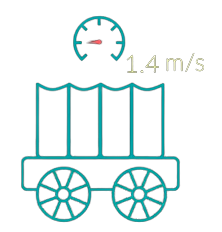
\includegraphics[width = \textwidth]{img/wagon.png}
        \end{minipage}
        \begin{minipage}{0.75\textwidth}
            There is a wagon travelling at a non-constant speed $v(t)$ (m/s) starting from an initial time $t = 0$. \textbf{What distance $\pmb{s(t)}$ will the wagon have traveled after $\pmb{t}$ units of time?}

            Conversely, if you are given the distance curve $s(t)$, what is the velocity function $v(t)$?
        \end{minipage}
    \end{block}

    % \begin{block}{Solution (Nicole Oresme (French philosopher 1320-1325 – 1382))}
    %     \begin{minipage}{0.29\textwidth}
    %         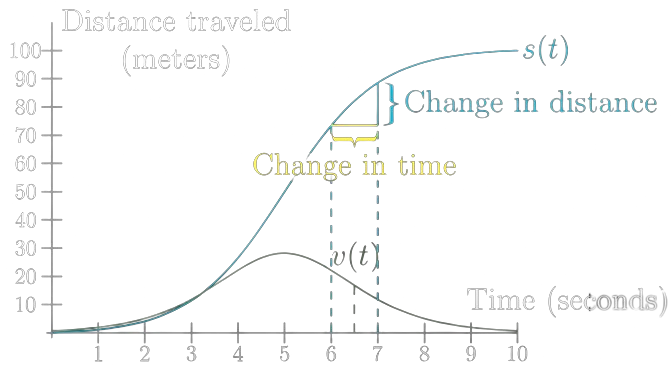
\includegraphics[width = \textwidth, height = 4cm]{img/velocity-distance.png}
    %     \end{minipage}
    %     \begin{minipage}{0.67\textwidth}

    %         \begin{enumerate}[leftmargin = 0.3cm, label = $\bullet$, rightmargin = 0cm]
            
    %         \item The question is about the relation between the velocity and distance curves

    %         \item Assume constant speed $v(t_1)$ in the segment $(0, t_1)$, $v(t_2)$ in the segment $(t_1, t_2)$, $\dots$

    %         \item \mbox{$s(t_n) \approx v(t_1)(t_1 - 0) + v(t_2)(t_2 - t_1) + \cdots + v(t_n)(t_n - t_{n-1})$} \\
    %         $\approx$ area under the curve $s(t)$ from $t = 0$ to $t = t_n$

    %         \item Conversely, $v(t_n) \approx (s(t_{n+1}) - s(t_n)) / (t_n - t_{n-1})$

    %         \end{enumerate}
            
    %     \end{minipage}
    % \end{block}
    
    

%     % : Given an object traveling for some period of time with nonuniform velocity, and given a velocity-time graph of said object’s motion, the displacement of this object will be proportional to the area under the curve of that velocity-time graph. 
    
    
\end{frame}

\begin{frame}{Pre-calculus}

    \centering
    Before diving into calculus we need to introduce other basic concepts, \\
    like the \textbf{limits of functions} and some of their \textbf{analytical properties}, \\ and the \textbf{notion of infinitesimal}
    
\end{frame}
%----------------------- INTRODUCTION -----------------------%

%----------------------- LIMITS OF FUNCTIONS -----------------------%
\section{Limits of functions, continuity and monotonocity}

\begin{frame}{Limits of functions}

    % Like sequences (output) approach terminal value when the index (input) increases, functions can return numbers (output) arbitrarily close to a value when their arguments (input) approaches a point
    \vspace{0.1cm}
    
    \begin{block}{Limit of a function from $\R$ to $\R$. three equivalent definitions}

        The real-valued function $f(x)$, with $x\in\R$, has limit $l$ at $x = a$, denoted by $\lim_{x\rightarrow a}f(x) = l$, iff
        
        \begin{enumerate}[leftmargin = 0.5cm, label = $\bullet$, rightmargin = 0.2cm]

            \item \textbf{Informal definition:} $f(x)$ gets closer to $l$ as $x$ gets closer to $a$

            % \item \textbf{Formal definition:} For all $\varepsilon > 0$, there exist $\delta > 0$ such that $|f(x) - l| \leq \varepsilon$ whenever $|x - a| < \delta$

            \item \textbf{Sequence-based definition:} For every sequence $x_n$ that converges to $a$, the resulting sequence $f(x_n)$ converges to $l$

            \item \textbf{Left-right limits definition:} The \orange{limit from the left and from the right} of $f(x)$ at $x = a$ are both equal to $l$
                    
        \end{enumerate}
        
    \end{block}

    \begin{minipage}{0.65\textwidth}
        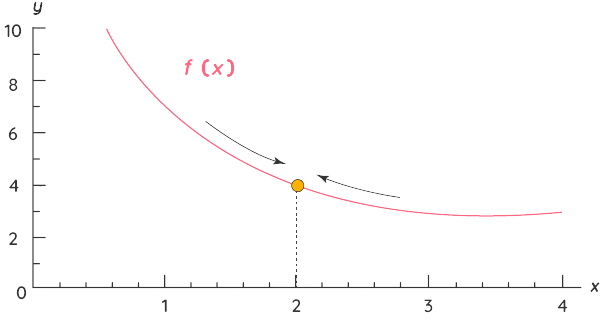
\includegraphics[width = \textwidth, height = 2.8cm]{img/limit-function.png}
    \end{minipage}\hspace{0.25cm}
    \begin{minipage}{0.3\textwidth}
        \centering
        \orange{What are these} \\ \orange{left and right limits?}
    \end{minipage}
    
    
\end{frame}

\begin{frame}{Left and right limits of a function}

    {\hspace{0.05cm}
    \begin{minipage}{0.45\textwidth}
        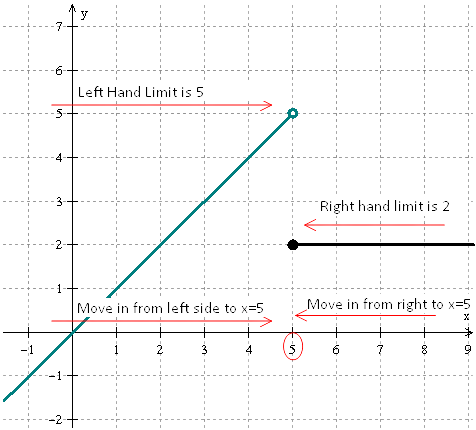
\includegraphics[width = 0.9\textwidth, height = 6cm]{img/left-right.limit.png}
    \end{minipage}
    \begin{minipage}{0.52\textwidth}
    \vspace{-0.1cm}
    
    \begin{block}{Limits from the left and from the right \\ Two equivalent definitions}
        The \blue{left} (\orange{right}) limit of $f(x)$ at $x = a$ equals $l$, denoted by \\ 
        \blue{$\lim_{x\uparrow a}f(x) = l$ or $\lim_{x\rightarrow a^-}f(x) = l$} \\
        (\orange{$\lim_{x\downarrow a}f(x) = l$ or $\lim_{x\rightarrow a^+}f(x) = l$}), iff
        \vspace{0.2cm}
        
        \begin{enumerate}[leftmargin = 0.5cm, label = $\bullet$, rightmargin = 0.2cm]

            \item \textbf{Informal definition:} $f(x)$ gets closer to $l$ as $x$ gets closer to $a$ by only taking values \blue{lower} (\orange{greater}) than $a$

            % \item \textbf{Formal definition:} For all $\varepsilon > 0$, there exist $\delta > 0$ such that $|f(x) - l| \leq \varepsilon$ whenever \blue{$0 < a - x < \delta$} (\orange{$0 < x - a < \delta$})

            \item \textbf{Sequence-based definition:} For every sequence $x_n$ that converges to $a$ and such that \blue{$x_n \leq a$} (\orange{$x_n \geq a$}) for all $n\in\N$, the resulting sequence $f(x_n)$ converges to $l$
        
        \end{enumerate}
    \end{block}
        
    \end{minipage}
    }
    
\end{frame}

\begin{frame}{Continuity of a function}

    \vspace{0.3cm}

    
    \begin{block}{Intuition of continuity}
        Roughly speaking, a function is continuous if \textbf{small changes in the input result in small changes in the output}

        Visually, the graph of a continuous function is connected, that is, it has no breaks
    \end{block}
    
    \begin{block}{Definition of continuity (and discontinuity)}
    
        \begin{enumerate}[leftmargin = 0.5cm, label = $\bullet$, rightmargin = 0.2cm]
        
        \item A function $f(x)$ is \textbf{continuous} at $x = a$ iff $\lim_{x\rightarrow a}f(x) = f(a)$

        \item A function $f(x)$ is \textbf{discontinuous} at $x = a$ iff it is not continuous at $x = a$

        \item A function is continuous in $I \subset \R$ if it is continuous at every point of $I$

        \item A function is continuous if it is continuous at every point of its domain

        \item A function $f$ is continuous from the \blue{left} (\orange{right}) at $x = a$ iff \\
        \blue{$\lim_{x\rightarrow a^-}f(x) = f(a)$} (\orange{$\lim_{x\rightarrow a^+}f(x) = f(a)$})
        
        \end{enumerate}
    \end{block}
    \vspace{-0cm}

\end{frame}

\begin{frame}{Continuity of a function}

    \begin{center}
        \textbf{Continuous vs Discontinuous}
    \end{center}
    \vspace{-0.7cm}
    
    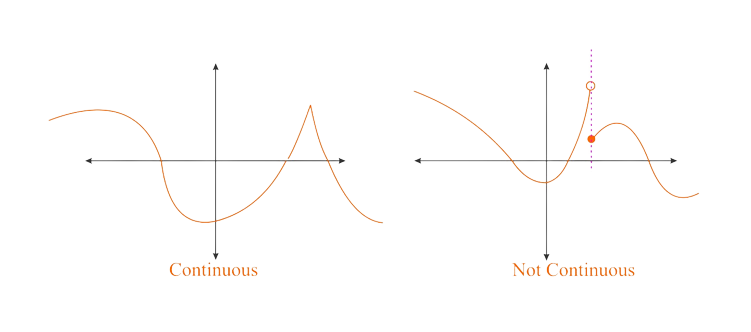
\includegraphics[width = \textwidth, height = 4cm]{img/continuous-vs-discontinuous.png}
    \vspace{-0.4cm}
    
    \begin{center}
        \textbf{Types of discontinuities}
    \end{center}
    \vspace{-0.4cm}
    
    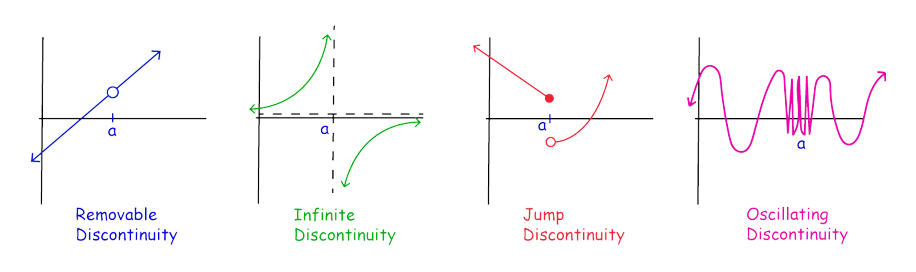
\includegraphics[width = \textwidth]{img/types-of-discontinuity.png}
    
\end{frame}

\begin{frame}{Preservation of continuity}

    If $f$ and $g$ are continuous functions
    \begin{enumerate}[leftmargin = 0.5cm, label = $\bullet$, rightmargin = 0.2cm]
        \item $f\pm g$ is continuous
        \item $fg$ is continuous
        \item $f/g$ is continuous at every point such that $g(x)\neq 0$
        \item $f^r$ is continuous for all $r\in\R$ (whenever it is well defined)
        \item The inverse of $f$, if it exists, is continuous
        \item $f\circ g$ is continuous (if the composition can be made)
    \end{enumerate}

    \begin{block}{Examples}
        By using the above properties of continuous functions, we can prove that
        \begin{enumerate}[leftmargin = 0.5cm, label = $\bullet$, rightmargin = 0.2cm]
            \item Polynomials are continuous
            \item Quotients of polynomials are continuous for every point that does not vanish the denominator
        \end{enumerate}
    \end{block}
    
\end{frame}

\begin{frame}{Monotonicity of a function}

    \begin{block}{Increasing and decreasing function. Three equivalent definitions}
        \ A function $f(x)$ with domain $D\subset \R$ is said to be \blue{\textbf{increasing}} (\orange{\textbf{decreasing}}) on the interval $I \subset D$ iff

        \begin{enumerate}[leftmargin = 0.5cm, label = $\bullet$, rightmargin = 0.2cm]

            \item \textbf{Informal definition:} $f$ produces \blue{lower} outputs for \blue{lower} (\orange{greater}) inputs in $I$
            %In the proximity of $x = a$, \\
            %$f(x)$ is \blue{lower} (\orange{greater}) or equal than $f(a)$ if $x$ is \blue{lower} (\orange{greater}) or equal than $a$, and \\
            % $f(x)$ is \blue{greater} (\orange{lower}) or equal than $f(a)$ if $x$ is \blue{greater} (\orange{lower}) or equal than $a$

            \item \textbf{Formal definition:} $\blue{f(x_1) \leq f(x_2)}$ (\orange{$f(x_1) \geq f(x_2)$}) whenever $x_1 \leq x_2$, with $x_1, x_2 \in I$
            % There exists $\varepsilon > 0$ such that $ \blue{f(x) \leq f(a) \leq f(y)}$ ($\orange{f(x) \geq f(a) \geq f(y)}$) whenever $x\in (a - \varepsilon, a) \cap D$ and $y \in (a, a + \varepsilon)\cap D$
            
        \end{enumerate}

        \begin{enumerate}[leftmargin = 0.8cm, label = (\textit{\roman*}), rightmargin = 0.2cm]
            \item If the inequalities are strict, $f$ is said to be \textbf{strictly} \blue{increasing} (\orange{decreasing})
            
            % \item $f$ is \blue{increasing} (\orange{decreasing}) in $I\subset D$ if it so at every point in $I$ %\blue{increasing} (\orange{decreasing}) at every point in $I$

            \item $f$ is said to be \blue{increasing} (\orange{decreasing}) if it is so in its domain % \blue{increasing} (\orange{decreasing}) at every point of its domain $D$

            \item $f$ is \textbf{monotone} or \textbf{constant} if it is increasing and decreasing simultaneously, \\
            or, equivalently, if the output remains the same for every value of $x$
        \end{enumerate}
    \end{block}

    We will see a different way of assessing monotonicity in the differential calculus part
    
\end{frame}

\begin{frame}{Visualizing increasing, decreasing, and constant functions}

    {\hspace{0.3cm} 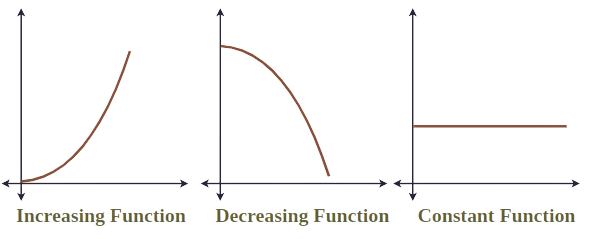
\includegraphics[width = 0.95\textwidth]{img/increase-decreasing.png}}
    
\end{frame}

\begin{frame}{Limits, continuity, and monotonicity of functions. An example}

    Examine the continuity and monotonicity of this function, as well as its limits when $x \rightarrow \infty$ and $x\rightarrow -3^+$
    \begin{align*}
        f(x) &= 
        \begin{cases}
            \frac{1}{x^3 + 27}, & \text{ if } x \in (-3, 0) \\
            2x, & \text{if } x \in [0, 10] \\
            25 + (x - 10)^2, & \text{if } x \in (10, \infty)
        \end{cases}
    \end{align*}
    
\end{frame}

\begin{frame}{Limits, continuity and monotonicity of functions — Solution}

\textbf{Continuity \& limits}
\begin{itemize}[label=$\bullet$,leftmargin=0.55cm]
\item Continuous on each piece: $(-3,0)$, $[0,10]$, $(10,\infty)$.
\item At $x=0$: $\displaystyle \lim_{x\to 0^-}\!f(x)=\frac1{27}\neq f(0)=0$ $\Rightarrow$ jump $\Rightarrow$ discontinuous.
\item At $x=10$: $\displaystyle \lim_{x\to 10^-}\!f(x)=20\neq \lim_{x\to 10^+}\!f(x)=25$ $\Rightarrow$ jump $\Rightarrow$ discontinuous.
\item $\displaystyle \lim_{x\to -3^+} f(x)=\lim_{x\downarrow -3}\frac{1}{(x+3)(x^2-3x+9)}=+\infty$ \\
$\Rightarrow$ vertical asymptote at $x=-3$ from the right.
\item $\displaystyle \lim_{x\to\infty} f(x)=\lim_{x\to\infty}\!\big[25+(x-10)^2\big]=+\infty.$
\end{itemize}

\textbf{Monotonicity}
\begin{itemize}[label=$\bullet$,leftmargin=0.55cm]
\item For $x\in(-3,0)$: decreasing.
\item For $x\in[0,10]$: increasing 
\item For $x\in(10,\infty)$: increasing
\item Upward jump at $x=10$.
\end{itemize}
\end{frame}


\begin{frame}{Rules of limits}

    \begin{block}{Rules of limits}
        Let $l_1 = \lim_{x\rightarrow a}f_1(x)$ and $l_2 = \lim_{x\rightarrow a}f_2(x)$, then
        \begin{enumerate}[leftmargin = 0.5cm, label = $\bullet$, rightmargin = 0.2cm]

            \item $\lim_{x\rightarrow a} \lrc{bf_1(x)} = bl_1$
            
            \item $\lim_{x\rightarrow a} \lrc{f_1(x) \pm f_2(x)} = l_1 \pm l_2$

            \item $\lim_{x\rightarrow a} \lrc{f_1(x)f_2(x)} = l_1l_2$

            \item $\lim_{x\rightarrow a} \lrc{f_1(x)/f_2(x)} = l_1/l_2$, if $l_2 \neq 0$
            
            \item $\lim_{x\rightarrow a} \lrc{f_1(f_2(x))} = \lim_{x\rightarrow l_2}f(x)$ (if the composition can be made)
        \end{enumerate}
        
    \end{block}

    \textbf{Example}
        \begin{align*}
            \lim_{x\rightarrow 2}\lrc{\frac{x - 3}{x^3} + (x - 1)^{100}} &= \lim_{x\rightarrow 2}\frac{x - 3}{x^3} + \lim_{x\rightarrow 2}(x - 1)^{100} \\
            &= \frac{\lim_{x\rightarrow 2}\lrc{x - 3}}{\lim_{x\rightarrow 2}x^3} + (\lim_{x\rightarrow 2}\lrc{x - 1})^{100} \\
            &= \frac{\lim_{x\rightarrow 2}x - 3}{(\lim_{x\rightarrow 2}x)^3} + (\lim_{x\rightarrow 2} x - 1)^{100} = \frac{-1}{8} + 1^{100} = \frac{7}{8}
        \end{align*}       
    
\end{frame}

\begin{frame}{Determinate forms. Examples}

    In the following examples, {\bf $\pmb{0}$ represents an infinitesimal}, not the actual number zero
    \vspace{0.3cm}
    
    \begin{block}{Determinate forms}
    Determinate forms of limits refer to those cases in which the algebraic operations of limits of functions %, which either diverge or converge to zero, 
    are \textbf{well-defined}
        \begin{enumerate}[leftmargin = 0.5cm, label = $\bullet$, rightmargin = 0.2cm]
            
            \item $\infty + \infty = \infty$,\quad
            e.g, $\lim_{x\rightarrow 0} 1/x^2 + 1/\sin(x) = \infty$
            \item $\pm\infty^{\infty} = \pm\infty$,\quad
            e.g, $\lim_{x\rightarrow \pi/2} (1/\cos(x))^{1/(x-\pi/2)} = \infty$
            \item $\pm\infty^{-\infty} = 0$,\quad
            e.g, $\lim_{x\rightarrow \infty} \ln(x)^{-x} = 0$
            \item $\infty\times\infty = \infty$
            \item $\infty/0 = \infty$ or $-\infty$ or does not exist,\quad
            e.g, $\lim_{x\rightarrow 0} (1/x^2)/(x\sin(1/x))$ does not exist
            % \item $0\times 0 = 0$
            \item $0^\infty = 0$,\quad
            e.g, $\lim_{x\rightarrow \infty} (1/x)^x = 0$
            \item $0^{-\infty} = \infty$ or $-\infty$,\quad
            e.g, $\lim_{x\rightarrow 0} x^{-1/x^2} = \infty$
            
            \end{enumerate}
    \end{block}
    
\end{frame}

\begin{frame}{Indeterminate forms. Examples}

    In the following examples, {\bf $\pmb{0}$ and $\pmb{1}$ represent an infinitesimal and a sequence convergent to the number one}, not the actual numbers zero and one
    \vspace{0.3cm}
    
    \begin{block}{Indeterminate forms}
    Indeterminate forms of limits refer to those cases in which the algebraic operations of limits of functions %, which either diverge or converge to zero or one, 
    are \textbf{not well-defined}
            \begin{enumerate}[leftmargin = 0.5cm, label = $\bullet$, rightmargin = 0.2cm]
            
            \item $\infty/\infty$,\quad
            e.g, $\lim_{x \rightarrow \infty }\frac{4x + 1}{2x} = 2$, $\lim_{x\rightarrow \infty }\frac{4x^2 + 1}{2x} = \infty$
            \item $\infty - \infty$,\quad
            e.g, $\lim_{x\rightarrow 0} (x^{-4} - x^{-2}) = \infty$
            \item $1^\infty$,\quad
            e.g, $\lim_{x\rightarrow \infty} (1 + 1/x)^x = e$
            \item $\infty^0$,\quad
            e.g, $\lim_{x\rightarrow \infty} (10^x)^{1/x} = 10$, $\lim_{x\rightarrow \infty} (10^{x^2})^{1/x} = \infty$
            \item $0/0$,\quad 
            % $\lim_{x\rightarrow0} \sin(x)/x = 1$, $\lim_{x\rightarrow\infty} \ln(1/2^x)/x^2$
            e.g, $\lim_{x\rightarrow 3}(x^2-9)^2/(x-3) = 6$, $\lim_{x\rightarrow 0} (x^2 - 1)/(x^2 - 2x + 1) = \infty$
            \item $0^0$,\quad e.g, $\lim_{x\rightarrow\infty} x^{1/\ln(x)} = e$
            
            \item $0\times\infty$,\quad
            $\lim_{x\rightarrow\frac{\pi}{2}^-} \tan(x)\cos(x) = 1$, $\lim_{x\rightarrow \infty} \tan(x)\cos(x)$ \text{does not exists}
            
            \end{enumerate}
    \end{block}

    \begin{center}
    {\tiny
    There is a powerful technique (called LH'ôpital's rule) to solve indeterminate forms. 
    Unfortunately, we won't see it in this course
    }    
    \end{center}
    
    
\end{frame}

% \begin{frame}{A note on infinitesimals}

%     Like infinite, an \textbf{infinitesimal} is not a number, but a concept. It represents a quantity closer to zero than any number, or a sequence of numbers that converge to zero

%     Also like infinite, the notion of infinitesimal has challenged intuition and rigor in Mathematics 
    
%     \begin{block}{Conterintuition examples}
        
%         \begin{itemize}[leftmargin = 0.5cm, label = $\bullet$, rightmargin = 0.2cm]
        
%         \item \textbf{Zeno's Paradoxes:} Achilles races a turtle but gives it a head start. Since Achilles must reach the turtle's starting point first, and then the turtle moves slightly, this process repeats infinitely, seemingly preventing Achilles from ever overtaking the turtle

%         \end{itemize}
%     \end{block}

%     % \begin{minipage}{0.48\textwidth}
%     %     
\includegraphics[width = 0.9\textwidth, height = 2cm]{img/infinite.png}
%     % \end{minipage}
%     % \begin{minipage}{0.47\textwidth}
%     %     \begin{block}{Indeterminate forms}
%     %         $\infty/\infty$,\ $\infty - \infty$, $1^\infty$, $\infty^0$, $0/0$, $0^0$, $0\times\infty$
%     %     \end{block}
%     % \end{minipage}
    
% \end{frame}

\begin{frame}{$\pmb{0/0}$ and $\pmb{\infty\times 0}$: the germ of calculus}

    We will see next...
    \vspace{0.3cm}
    
    ... how the study of indeterminate forms of the type $0/0$ leads to \textbf{differential calculus}...
    \vspace{0.3cm}
    
    ... and how the study of $0\times\infty$ leads to \textbf{integral calculus}
    
\end{frame}
%----------------------- LIMITS OF FUNCTIONS -----------------------%


\section{Differential calculus of one-variable functions}

\begin{frame}{The derivative paradox: an instantaneous rate of change}

    \begin{enumerate}[leftmargin = 0.5cm, label = $\bullet$, rightmargin = 0.2cm]
        
        \item Think about the speedometer of your car 
    
        \item What does it mean that you are moving at $60$km/h at a given moment $t$?

        \item   \begin{minipage}{0.45\textwidth}
                    Tell me how fast this car is moving 
                \end{minipage}
                \begin{minipage}{0.45\textwidth}
                    {\hspace{-0.3cm} 
\includegraphics[width = 0.5\textwidth]{img/car.png}}
                \end{minipage}

        \item You can't, because it's not moving

        \item So, how does the speedometer tell you that you are moving at $60$km/h at time $t$?

        \item It uses the velocity formula\footnote{What it actually does is measuring the rotation of the wheels, which is equivalent} (distance/time) in a small time interval $(t, t + \Delta t)$: 
        $$
        \frac{\text{distance traveled from } t \text{ to } t + \Delta t}{\Delta t}
        $$

        \item But this is not an instantaneous velocity, isn't it?

        \item It is not, but, in mathematics, we have the advantage of infinitesimals
    \end{enumerate}
    
\end{frame}

\begin{frame}{Derivative as velocity}

%------------------ LEFT: TABLE ------------------
\begin{enumerate}[leftmargin=0.5cm, label=$\bullet$, rightmargin=0.2cm]
  \item Imagine that, after $t$ hours you have driven for $s(t)=t^2$ km.
  \item What is the speed at $t = 2$?
  \item Approximate by average speed:
  $
    \frac{\Delta s}{\Delta t} = \frac{s(2+\Delta t)-s(2)}{\Delta t}
  $
  \item Compute it for smaller and smaller (in absolute value) $\Delta t$:
\end{enumerate}
% \medskip
\begin{center}
\begin{tabular}{r c}
\textbf{$\Delta t$} & \textbf{$\Delta s/\Delta t$}\\
\hline
$1$      & $5.00$\\
$0.5$    & $4.50$\\
$0.1$    & $4.10$\\
$0.01$   & $4.01$\\
${-}0.1$  & $3.90$\\
${-}0.01$ & $3.99$
\end{tabular}    
\end{center}
\begin{enumerate}[leftmargin=0.5cm, label=$\bullet$, rightmargin=0.2cm]
\item Can you spot the limit as $\Delta t \rightarrow 0$?
\item For a general $\Delta t$:
$
\frac{s(2+\Delta t)-s(2)}{\Delta t}
=\frac{(2+\Delta t)^2-4}{\Delta t}
=4+\Delta t
$
\end{enumerate}
$$
\boxed{\,v(2)=\lim_{\Delta t\to 0}\frac{s(2+\Delta t)-s(2)}{\Delta t}=4\ \text{km/h}\,}
$$

\end{frame}


\begin{frame}{Differential of a one-variable function: the derivative}

    \begin{minipage}{0.45\textwidth}
    
        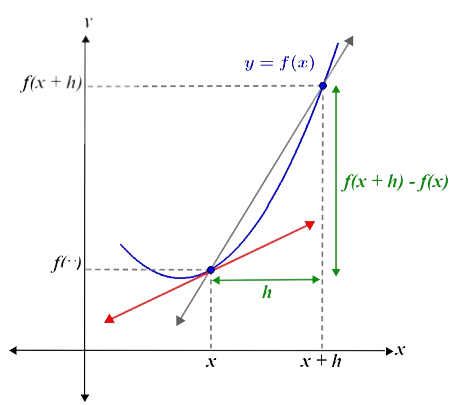
\includegraphics[width = \textwidth, height = 4.5cm]{img/derivative-tangent.png}
        
    \end{minipage}\hspace{0.2cm}
    \begin{minipage}{0.5\textwidth}
        \vspace{0cm}
        
        \begin{block}{Definition of the derivative of a function}
            The derivative of a real-valued function $f(x)$, with $x\in \R$, is defined as
            $$
            f'(x) := \lim_{\Delta x\rightarrow 0} \frac{f(x + \Delta x)-  f(x)}{\Delta x} = \lim_{\Delta x\rightarrow 0}\frac{\Delta f}{\Delta x}
            $$
            \textbf{Intuition:} How an infinitesimal change in the function's input affects the output?
        \end{block}

        
    \end{minipage}

    % \begin{block}{Derivatives as slopes of tangents}
    %         It easily comes from the definition of derivatives that the tangent line of a function $f(x)$ at $x = a$ is given by
    %         $$
    %         m(x) = f'(a)(x - a) + f(a)
    %         $$
    % \end{block}

    % \begin{block}{Derivability implies continuity}
    %     If $f(x)$ is derivable at $x = a$, then it is continuous at the same point
    % \end{block}
    
\end{frame}

\begin{frame}{The derivative as the slope of the tangent line}

    \begin{center}
        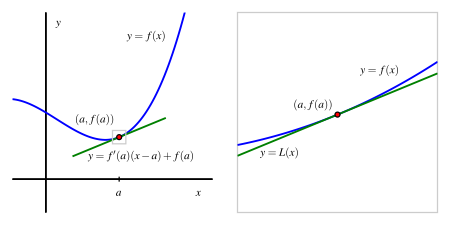
\includegraphics[width = 0.7\textwidth]{img/TanLine.png}
    \end{center}
    \medskip
     
    \begin{block}{Derivatives as slopes of tangents}
            It easily comes from the definition of derivatives that the tangent line of a function $f(x)$ at $x = a$ is given by
            $$
            m(x) = f'(a)(x - a) + f(a)
            $$
    \end{block}

    \begin{center}
        \href{https://www.geogebra.org/m/WGCsKBeM?utm}{Visualize here!} \hspace{1cm}
        \href{https://www.desmos.com/calculator/lxyh9tqd5d}{And here!}
    \end{center}
    % \begin{block}{Derivability implies continuity}
    %     If $f(x)$ is derivable at $x = a$, then it is continuous at the same point
    % \end{block}
    
\end{frame}

\begin{frame}{Computing derivatives. Example}

  \begin{block}{The derivative of $f(x) = \pmb{\sqrt{x}}$\ (for $x>0$)}
    \begin{align*}
      f'(x) &= \lim_{h\to 0}\frac{\sqrt{x+h}-\sqrt{x}}{h} \\[2pt]
      &= \lim_{h\to 0}\frac{\sqrt{x+h}-\sqrt{x}}{h}
         \cdot \frac{\sqrt{x+h}+\sqrt{x}}{\sqrt{x+h}+\sqrt{x}}
         \quad \text{\small(conjugate)} \\[2pt]
      &= \lim_{h\to 0}\frac{(x+h)-x}{h\big(\sqrt{x+h}+\sqrt{x}\big)} \\[2pt]
      &= \lim_{h\to 0}\frac{1}{\sqrt{x+h}+\sqrt{x}}
       \;=\; \frac{1}{2\sqrt{x}} \, .
    \end{align*}
  \begin{scriptsize}
    \emph{Note.} The formula holds for $x>0$. At $x=0$ the derivative does not exist (see next slide).
  \end{scriptsize}
  \end{block}

Later, we will introduce \textbf{techniques for fast and easy derivative computation}, avoiding this direct, cumbersome method

\end{frame}


% \begin{frame}{Computing derivatives. Examples}

%     \begin{block}{The derivative of $\pmb{x^2}$}
%         \begin{align*}
%             \lim_{h\rightarrow 0}\frac{(x + h)^2 - x^2}{h} &= 
%             \lim_{h\rightarrow 0}\frac{x^2 + 2xh + h^2 - x^2}{h} \\
%             &= \lim_{h\rightarrow 0}\frac{2xh + h^2}{h} \\
%             &= \lim_{h\rightarrow 0}2x + h = 2x
%         \end{align*}
%     \end{block}
    
% \end{frame}

\begin{frame}{Example of cases where the derivative does not exist}

    \begin{block}{$\pmb{f(x) = |x|}$ is not derivable at $\pmb{x = 0}$}
        \begin{align*}
            \lim_{h\rightarrow 0^+}\frac{f(0 + h) - f(0)}{h} & =
            \lim_{h\rightarrow 0^+}\frac{|h|}{h} = 1 \\
            \lim_{h\rightarrow 0^-}\frac{f(0 + h) - f(0)}{h} & =
            \lim_{h\rightarrow 0^-}\frac{|h|}{h} = -1
        \end{align*}
    \end{block}

    \begin{block}{$\pmb{f(x) = \sqrt{x}}$ is not derivable at $\pmb{x = 0}$}
        \begin{align*}
            \lim_{h\rightarrow 0^+}\frac{f(0 + h) - f(0)}{h} & =
            \lim_{h\rightarrow 0^+}\frac{ \sqrt{h}}{h} \\
            &= \lim_{h\rightarrow 0^+}\frac{1}{\sqrt{h}} = \infty
        \end{align*}
    \end{block}
    
\end{frame}

\begin{frame}{Derivatives as the impact of small perturbations}

    \vspace{0.2cm}
    
    \begin{enumerate}[leftmargin = 0.5cm, label = $\bullet$, rightmargin = 0.2cm]
    
    \item An application of the derivative of a function, $f'(x)$, is to (linearly) \textbf{approximate how small changes in the input affects the output}

    \item Indeed, Since $f'(x)$ is the limit of $f(x + \Delta x) - f(x)$ as $\Delta x$ approaches zero, for small values of $\Delta x$,
    $$
    f'(x) \approx \Delta f/ \Delta x\ \Longleftrightarrow \Delta f \approx f'(x)\Delta x
    $$
    \end{enumerate}
    \vspace{0.2cm}
    
    {\hspace{2.6cm} 
    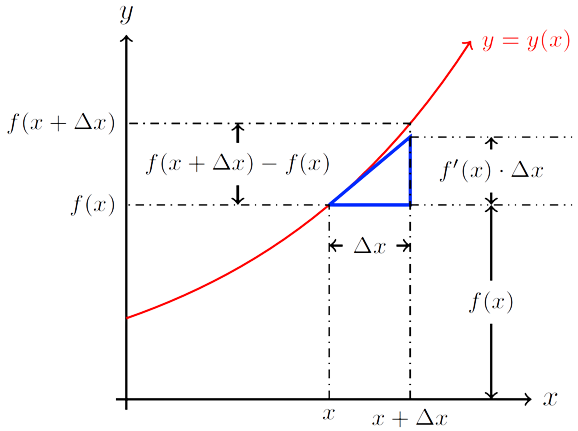
\includegraphics[width = 0.55\textwidth]{img/linear-approximation.png}
    }
    
    
    
\end{frame}

\begin{frame}{Derivatives as the impact of small perturbations. An example}

    \textbf{Example}
        \vspace{0.1cm}
        
        \begin{enumerate}[leftmargin = 0.8cm, label = (\alph*), rightmargin = 0.2cm]
            
            \item Find the equation of the tangent of the parabola $f(x) = x^2$ at $x = a$.
            
            \item Use the tangent to approximate the value $f(a + 0.1)$ and compute the error of approximation 
    
            \item Comment on why it is advantageous to use the derivative to approximate the impact of the perturbation rather than computing the exact perturbed output.
        \end{enumerate}
        
    
\end{frame}

\begin{frame}{Derivatives as the impact of small perturbations — Solution}

\textbf{Solution}
\begin{enumerate}[leftmargin=0.8cm, label=(\alph*), rightmargin=0.2cm]

\item For $f(x)=x^2$, $f'(x)=2x$. \\
Slope at $x=a$ is $2a$, so the tangent is
\[
y(t) = f(a)+f'(a)(t-a)=a^2+2a(t-a)=2at-a^2.
\]

\item Linear (tangent) approximation at $a$:
\[
f(a+0.1)\approx y(a+0.1) = a^2+2a(0.1).
\]
Exact value: $(a+0.1)^2=a^2+0.2a+0.01$. \\
\textbf{Error (exact $-$ approx)} $=0.01$.

\item Why useful: the derivative gives the best local linear approximation, 
which is fast to compute and, for small perturbations, is also accurate.

\end{enumerate}

\end{frame}


\begin{frame}{Differentiation rules}

    These properties of the differentiation operation are easily derived from its definition
    \begin{block}{Differentiation rules}
        
        \begin{enumerate}[leftmargin = 0.5cm, label = $\bullet$, rightmargin = 0.2cm]

        \item \textbf{Linearity:} \\
        $h(x) = a f(x) + b g(x) \Longrightarrow h'(x) = a f'(x) + b g'(x)$, for $a, b \in\R$

        \item \textbf{Product rule:} \\
        $h(x) = f(x)g(x) \Longrightarrow h'(x) = f'(x)g(x) + f(x)g'(x)$

        \item \textbf{Quotient rule:} \\ 
        $h(x) = f(x)/g(x) \text{ and } g'(x) \neq 0 \Longrightarrow h'(x) = \frac{f'(x)g(x) - f(x)g'(x)}{g(x)^2}$

        \item \textbf{Chain rule:} \\
        $h(x) = g(f(x)) \Longrightarrow h'(x) = g'(f(x))f'(x)$

        \item \textbf{Inverse rule:} \\
        $h(x) = f^{-1}(y) \Longrightarrow h'(y) = 1/f'(f^{-1}(y))$
        
        \end{enumerate}
        
    \end{block}
    
\end{frame}

\begin{frame}{Derivative of usual functions}

    These are the derivatives of the most common functions used in mathematics
    
    \begin{block}{Derivative of usual functions}

        \begin{enumerate}[leftmargin = 0.5cm, label = $\bullet$, rightmargin = 0.2cm]

        \item \textbf{Constant:} \\
        $f(x) = a,\; a \in\R \Longrightarrow f'(x) = 0$
        
        \item \textbf{Power:} \\
        %If either $a\in\R$ and $x\in\R_+$ or $a\in\Z$ and $x\in\R$, then 
        $f(x) = x^a \Longrightarrow f'(x) = a x^{a-1}$
        

        \item \textbf{Exponential:} \\
        $f(x) = e^x \Longrightarrow f'(x) = e^x$

        \item \textbf{Logarithm:} \\
        $f(x) = \ln(x) \Longrightarrow f'(x) = 1/x$

        \item \textbf{Trigonometric:} \\
        $f(x) = \sin(x),\; g(x) = \cos(x) \Longrightarrow f'(x) = \cos(x),\; g'(x) = -\sin(x)$
        
        \end{enumerate}
        
    \end{block}
    
\end{frame}

\begin{frame}{Computing derivatives. Example 1: linearity}

        Let $f(x) = -2\ln(x) + 3x^5$. Compute $f'(x)$

        \begin{enumerate}[leftmargin = 0.5cm, label = \arabic*., rightmargin = 0.2cm]

        \item Note that $f$ is the linear combination of two functions: $f(x) = -2f_1(x) + 3f_2(x)$, with $f_1(x) = \ln(x)$ and $f_2(x) = x^5$

        \item Compute $f_1'(x)$ and $f_2'(x)$: $f_1'(x) = 1/x$ and $f_2'(x) = 5x^4$

        \item Compute $f'(x)$ by using the linearity of the derivative: $f'(x) = -2f_1'(x) + 3f_2'(x) = -2/x + 15x^4$ 
        
        \end{enumerate}
    
\end{frame}

\begin{frame}{Computing derivatives. Example 2: The product rule}

        Let $f(x) = (x^3 + 1)(x^2 + 5)$. Compute $f'(x)$

        \begin{enumerate}[leftmargin = 0.5cm, label = \arabic*., rightmargin = 0.2cm]

        \item Note that $f$ is the product of two functions: $f(x) = f_1(x)f_2(x)$, with $f_1(x) = (x^3 + 1)$ and $f_2(x) = x^2 + 5$

        \item Compute $f_1'(x)$ and $f_2'(x)$: $f_1'(x) = 3x^2$ and $f_2'(x) = 2x$

        \item Compute $f'(x)$ by using the product rule:
        \begin{align*}
            f'(x) = f_1'(x)f_2(x) + f_1(x)f_2'(x) = 3x^2(x^2 + 5) + (x^3 + 1)2x
        \end{align*} 
        
        \end{enumerate}
    
\end{frame}

\begin{frame}{Computing derivatives. Example 3: the quotient rule}

        Let $f(x) = \cos(x)/(x^2 + 5)$. Compute $f'(x)$

        \begin{enumerate}[leftmargin = 0.5cm, label = \arabic*., rightmargin = 0.2cm]

        \item Note that $f$ is the quotient of two functions: $f(x) = f_1(x)/f_2(x)$, with $f_1(x) = \cos(x)$ and $f_2(x) = x^2 + 5$

        \item Compute $f_1'(x)$ and $f_2'(x)$: $f_1'(x) = -\sin(x)$ and $f_2'(x) = 2x$

        \item Compute $f'(x)$ by using the quotient rule: 
        \begin{align*}
            f'(x) = \frac{f_1'(x)f_2(x) - f_1(x)f_2'(x)}{(f_2(x))^2} = \frac{-\sin(x)(x^2 + 5) -2x\cos(x)}{(x^2 + 5)^2}
        \end{align*} 
        
        \end{enumerate}
    
\end{frame}

\begin{frame}{Computing derivatives. Example 4: the chain rule}

        Let $f(x) = \ln(x^2 + 2)$ and $g(x) = x^4 + x^{-2}$. Compute $(f\circ g)'(x)$

        \begin{enumerate}[leftmargin = 0.5cm, label = \arabic*., rightmargin = 0.2cm]

        \item Compute $f'(x)$: Note that $f(x) = f_1(f_2(x))$, for $f_1(x) = \ln(x)$ and $f_2(x) = x^2 + 2$. Hence,
        \begin{align*}
             f_1'(x) &= 1/x; \quad f_2'(x) = 2x \\
            \Longrightarrow f'(x) &= f_1'(f_2(x))f_2'(x) = \frac{1}{x^2 + 2}2x,
        \end{align*}
        where the implication comes after the chain rule

        \item Compute $g'(x)$: The linearity of the derivative operator alongside the power rule gives us that $g'(x) = 4x^3 - 2x^{-3}$.

        \item Compute $(f\circ g)'(x)$: Finally, use the previous results and apply again the chain rule to obtain        
        \begin{align*}
            (f\circ g)'(x) = f'(g(x))g'(x) = \frac{2(x^4 + x^{-2})}{(x^4 + x^{-2})^2 + 2}(4x^3 - 2x^{-3})
        \end{align*}
        
        \end{enumerate}
    
\end{frame}

% \begin{frame}{Economical application: cost, profit, and revenue}

%     \begin{enumerate}[leftmargin = 0.5cm, label = , rightmargin = 0.2cm]
%         \item \textbf{Cost function:} $C(q) = $ how much it costs to a company to produce $q$ units of a product

%         \item \textbf{Revenue function:} $R(q, p) = qp$ how much a company makes by selling  $q$ units of a product at $p$ dollars each unit

%         \item \textbf{Profit function:} $P(q, p) = R(q, p) - C(q)$ net income a company makes by producing $q$ units of a product and selling them at $p$ dollars each unit
%     \end{enumerate}
    
% \end{frame}

\begin{frame}{Economical application: derivatives as marginal costs}

    \begin{enumerate}[leftmargin = 0.5cm, label = , rightmargin = 0.2cm]

        \item \textbf{Cost function:} $C(q) = $ how much it costs for a company to produce $q$ units of a product

        \item \textbf{Question:} How much more does a company have to pay to produce $q + \Delta q$ units given that it has already produced $q$ units?
        
        \item \textbf{Marginal cost:} $MC(q) = $ Difference between the cost of $q + \Delta q$ units and $q$ units,
        \begin{align*}
            MC(q) = C(q + \Delta q) - C(q) \approx C'(q)\Delta q
        \end{align*}
        (That is why, in economic lingo, ``marginal'' refers to derivatives, especially because economists often take $\Delta q = 1$, that is unit increment in production)
        
        %In order to produce $q$ units of an item, a company has to payout $C(q)$ dollars. That is, $C$ is the company's cost function. 
    
        % \item Economics uses the word ``marginal'' to describe a small change in production from $q$ to $q + \Delta q$. 
    
        % \item The corresponding increase in cost, $\Delta C = C(q + \Delta q) - C(q)$ is called the ``marginal cost'' (of making $\Delta q$ more unit) when the level of production is $q$. 
    
        % \item Hence, $\Delta C \approx C'(q)\Delta q$.

        % \item 
    \end{enumerate}
    
\end{frame}

\begin{frame}{The monotonicity of a function according to its derivative}

    \begin{block}{Increasing and decreasing according to the derivative}
        Let $I\subset\R$ be an \red{open interval}. Then,
        \begin{enumerate}[leftmargin = 0.5cm, label = $\bullet$, rightmargin = 0.2cm]
        
        \item $\blue{f'(x) \geq 0}$ ($\orange{f'(x) \leq 0}$) for all $x\in I\subset\R \Longrightarrow f$ is \blue{increasing} (\orange{decreasing}) in $I$

        \item $f'(x) = 0$ for all $x\in I\subset\R \Longrightarrow f$ is constant (monotone) in $I$
        
        \end{enumerate}

        If the inequalities are strict, $f$ is said to be strictly \blue{increasing} (\orange{decreasing})
        
    \end{block}
    \vspace{-0.2cm}

    \red{Note} that we asked for $I$ to be an open interval. This is to avoid $I$ being a single point, since the notion of pointwise monotonicity is a tricky one and it is safer to introduce the concept globaly. \textbf{Example:} $f(x) = x^3$ at $x = 0$, and $f(x) = x^2$ at $x = 0$
    \vspace{0.3cm}
    
    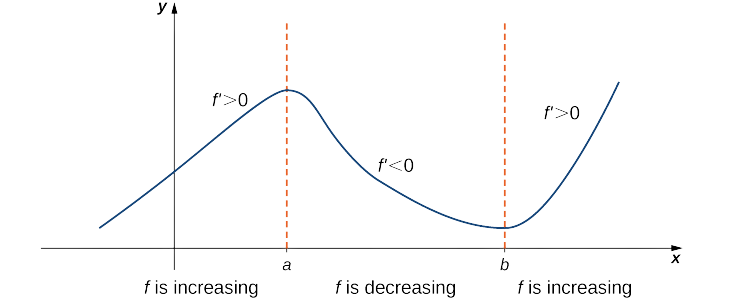
\includegraphics[width = \textwidth, height = 3.3cm]{img/increasing.decreasing.derivative.png}
    
\end{frame}

\begin{frame}{Economical application: elasticity of demand}

    \begin{enumerate}[leftmargin = 0.5cm, label = , rightmargin = 0.2cm]

        \item \textbf{Revenue as a function of price:} $R(p) = Q(p)p = $ how much a company makes by selling $Q(p)$ units of a product at $p$ dollars each unit

        \item \textbf{Question:} Will revenue increase if the selling price slightly increases?

        \item \textbf{Marginal Revenue:} By applying the product rule we can compute the derivative of the revenue function and answer the question
        \begin{align*}
            R'(p) = Q'(p)p + Q(p) > 0 \Longleftrightarrow - \frac{Q'(p)p}{Q(p)} < 1
        \end{align*}
        
        \item \textbf{Elasticity of Demand:} $\varepsilon(p) := -\frac{Q'(p)p}{Q(p)}$

        \item \textbf{Take away:}

        \begin{enumerate}[leftmargin = 0.5cm, label = $\bullet$, rightmargin = 0.2cm]
            
            \item Inelastic Demand ($\varepsilon(p) < 1$): a small increase in price results in an increase in revenue

            \item Elastic Demand: ($\varepsilon(p) > 1$): a small increase in price results in a decrease in revenue
            
        \end{enumerate}
        % \item \textbf{Profit function:} $P(q, p) = R(q, p) - C(q)$ net income a company makes by producing $q$ units of a product and selling them at $p$ dollars each unit
    \end{enumerate}
    
\end{frame}

% \begin{frame}{L’Hôpital’s rule}

% We already saw how complicated could be handling indeterminate forms of limits. The L’Hôpital’s rule simplifies this endevour.
% \medskip

% \begin{block}{Rule}
% If $\displaystyle \lim_{x\to a}\frac{f(x)}{g(x)}$ is of type $0/0$ or $\infty/\infty$, and $f,g$ are differentiable near $a$ (except possibly at $a$), with $g'(x)\neq 0$ near $a$, then
% \[
% \lim_{x\to a}\frac{f(x)}{g(x)} \;=\; \lim_{x\to a}\frac{f'(x)}{g'(x)}
% \quad\text{(provided the right-hand-side limit exists (finite or } \pm\infty\text{))}
% \]
% \end{block}

% \begin{block}{How to use it?}
%     \begin{enumerate}[leftmargin=0.65cm, label=\textbullet, rightmargin=0.2cm]
%         \item Try simple algebra first (factor, rationalize, common denominator).
%         \item If still $0/0$ or $\infty/\infty$, apply L’Hôpital once and re-evaluate.
%         \item If still indeterminate, you may apply again.
%     \end{enumerate}
% \end{block}
    
% % \medskip

% \begin{center}
% \begin{scriptsize}
% There are techniques to convert other indeterminate forms to $0/0$ or $\infty/\infty$, to then rely on the L'Hôpital rule.
% \end{scriptsize}    
% \end{center}

% \end{frame}

% \begin{frame}{General L'Hôspital's rule}

%     \begin{block}{L'Hôspital's rule}
%         If two functions $f(x)$ and $g(x)$ 

%         \begin{enumerate}[leftmargin = 0.8cm, label = (\alph*), rightmargin = 0.2cm]

%             \item They are differentiable in an open interval $I$ containing $x = a$ or having $x = a$ as a boundary point, except possibly at $x = a$ ($a$ could be $\pm\infty$)
            
%             \item Both $\lim_{x\rightarrow a} f(x)$ and $\lim_{x\rightarrow a} g(x)$ are $0$ or $\pm\infty$

%             \item $g'(x) \neq 0$ for all $x\in I$ such that $x\neq a$

%             \item $\lim_{x\rightarrow a} \frac{f'(x)}{g'(x)} = l$, where $l$ can be finite or $\pm\infty$
        
%         \end{enumerate}

%         Then,
%         \vspace{-0.2cm}
%         $$
%         \lim_{x\rightarrow a} \frac{f(x)}{g(x)} = \lim_{x\rightarrow a}\frac{f'(x)}{g'(x)}
%         $$
        
%     \end{block}
    
% \end{frame}

% \begin{frame}{The L'Hôspital rule. Straightforward applications}
    
%     \begin{block}{Example. $0/0$}
%         Find the limit $\lim_{x\rightarrow 0}\frac{\sin(x)}{x}$. 
%         Since the functions $f(x) = \sin(x)$ and $g(x) = x$ satisfy conditions (a)-(d) of the L'Hôspital rule at $x = 0$, then % and $f'(x) = \cos(x)$ and $g'(x) = 1$, then
%         \vspace{-0.1cm}
%         $$
%         \lim_{x\rightarrow 0}\frac{\sin(x)}{x} = \lim_{x\rightarrow 0}\frac{f(x)}{g(x)} = \lim_{x\rightarrow 0}\frac{f'(x)}{g'(x)} = \lim_{x\rightarrow 0}\cos(x) = 1
%         $$
%     \end{block}

%     \begin{block}{Example. $\infty/\infty$}
%         Find the limit $\lim_{x\rightarrow \infty}\frac{\ln(x)}{x}$.
        
%         Since the functions $f(x) = \ln(x)$ and $g(x) = x$ satisfy conditions (a)-(d) of the L'Hôspital rule at $\infty$, then % and $f'(x) = \cos(x)$ and $g'(x) = 1$, then
%         \vspace{-0.1cm}
%         $$
%         \lim_{x\rightarrow \infty}\frac{\ln(x)}{x} = \lim_{x\rightarrow \infty}\frac{f(x)}{g(x)} = \lim_{x\rightarrow \infty}\frac{f'(x)}{g'(x)} = \lim_{x\rightarrow \infty}1/x = 0
%         $$
%     \end{block}
    
% \end{frame}

% \begin{frame}{The L'Hôspital rule applied to other indeterminate applications}

%     \begin{block}{Example. $0\times\infty$}
%         Find the limit $\lim_{x\rightarrow 0}\ln(x)x$.
        
%         Note that $\ln(x)x = \ln(x)/(1/x)$.
        
%         Since the functions $f(x) = \ln(x)$ and $g(x) = 1/x$ satisfy conditions (a)-(d) of the L'Hôspital rule at $x = 0$, then % and $f'(x) = \cos(x)$ and $g'(x) = 1$, then
%         \vspace{-0.1cm}
%         $$
%         \lim_{x\rightarrow 0}\ln(x)x = \lim_{x\rightarrow 0}\frac{f(x)}{g(x)} = \lim_{x\rightarrow 0}\frac{f'(x)}{g'(x)} = \lim_{x\rightarrow 0}\frac{1/x}{-1/x^2} = 0
%         $$
%     \end{block}
    
% \end{frame}

% \begin{frame}{The L'Hôspital rule applied to other indeterminate applications}

%     \begin{block}{Example. $\infty^0$}
%         Find the limit $\lim_{x\rightarrow \infty}x^{1/x}$
        
%         Note that $x^{1/x} = \exp(\ln(x^{1/x})) = \exp(\ln(x)/x)$

%         Since $e^x$ is continuous, $\lim_{x\rightarrow\infty} \exp(\ln(x)/x) = \exp(\lim_{x\rightarrow\infty}\ln(x)/x)$
        
%         Since the functions $f(x) = \ln(x)$ and $g(x) = x$ satisfy conditions (a)-(d) of the L'Hôspital rule at $\infty$, then % and $f'(x) = \cos(x)$ and $g'(x) = 1$, then
%         \vspace{-0.1cm}
%         $$
%         \lim_{x\rightarrow \infty}\frac{\ln(x)}{x} = \lim_{x\rightarrow \infty}\frac{f(x)}{g(x)} = \lim_{x\rightarrow \infty}\frac{f'(x)}{g'(x)} = \lim_{x\rightarrow \infty}1/x = 0
%         $$

%         Finally, $\lim_{x\rightarrow \infty}x^{1/x} = \exp(\lim_{x\rightarrow\infty}\ln(x)/x) = 1$
%     \end{block}
    
% \end{frame}

\begin{frame}{Higher-order derivatives}

    Note that $f'$ is a  function, so we can derivate it and come up with what is called \textbf{second-order derivative} or, plainly, second derivative, denoted by $f''$.
    \vspace{0.3cm}

    Repeating this operation of taking ``the derivative of the derivative'', we end up with the concept of \textbf{higher-order derivative}.
    \vspace{0.3cm}

    At some point, adding apostrophes is not feasible. Could you imagine how cumbersome the notation may get (e.g., for the 5th derivative $f'''''$)?
    \vspace{0.3cm}

    Therefore, we use the notation $f^{(n)}$ for \textbf{the derivative of order} $\pmb{n}$ (or $n$th derivative) of $f$, for $n\in\N$.
    
\end{frame}

\begin{frame}{Application of second-order derivatives. The convexity of a function.}

    \vspace{0.2cm}
    
    \begin{block}{Convexity of a function}
    \begin{minipage}{0.4\textwidth}
        \vspace{0cm}
        
        {\hspace{00cm}
        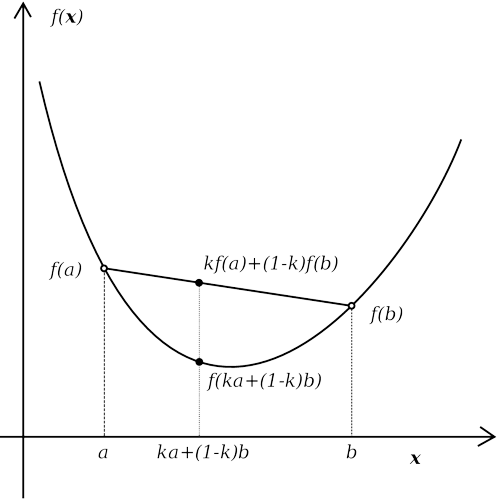
\includegraphics[width = 0.95\textwidth, height = 3.4cm]{img/convex-function.png}
        }
    \end{minipage}\hspace{0.1cm}
    \begin{minipage}{0.55\textwidth}
    \vspace{-0.3cm}
        
    A function $f$ is said to be \blue{convex} (\orange{concave}) iff, for all $k \in (0, 1)$ and all $a, b$ in the domain of $f$, 
    \begin{align*}
    \blue{f(k a + (1-k) b)}\ &\blue{\leq k f(a) + (1-k) f(b)} \\
    \pmb{(}\orange{f(k a + (1-k) b)}\ &\orange{\geq k f(a) + (1-k) f(b)}\pmb{)}    
    \end{align*}
    If the inequality is strict, the function is said to be strictly \blue{convex} (\orange{concave})

    \end{minipage}
    \end{block}

    The second derivative (the derivative of the derivative) of a function can be used to assess its convexity
    \begin{block}{Convexity of a function according to its second derivative}

        \begin{enumerate}[leftmargin = 0.5cm, label = $\bullet$, rightmargin = 0.2cm]
        
        \item $f''(x) \geq 0$ ($f''(x) \leq 0$) for all $x\in I \Longrightarrow f$ is  \blue{convex} (\orange{concave}) in $I$

         If the inequality is strict, the function is said to be strictly convex (concave)
        % \item $f'(x) \geq 0$ ($f'(x) < 0$) for all $x\in I \Longrightarrow f$ is (strictly) increasing in $I$

        \item $f''(x) = 0$ for all $x\in I \Longrightarrow f$ is both convex and concave in $I$, that is, $f$ is linear
        
        \end{enumerate}
        
    \end{block}
    
\end{frame}

\begin{frame}{Visualizing convexity. Examples}

    \begin{minipage}{0.48\textwidth}
        {\hspace{0.025cm}
        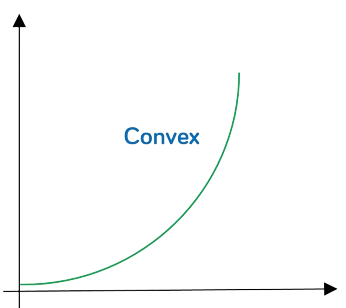
\includegraphics[width = \textwidth, height = 3.7cm]{img/convex.png}    
        }
    \end{minipage}
    \begin{minipage}{0.48\textwidth}
        \vspace{-0.1cm}
        
        {\hspace{0.5cm}
        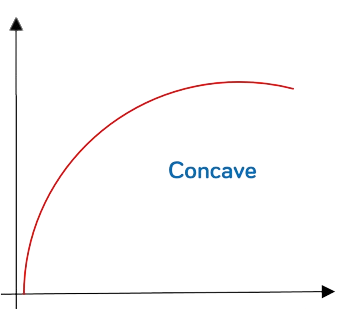
\includegraphics[width = \textwidth, height = 3.7cm]{img/concave.png}
        }
    \end{minipage}

    \begin{block}{Example}
        $f(x) = x^2 \Longrightarrow f''(x) = 2 > 0 \Longrightarrow f$ is convex.
    \end{block}

    \begin{block}{Example}
        $f(x) = \ln(x) \Longrightarrow f''(x) = -1/x^2 < 0 \Longrightarrow f$ is concave. 
    \end{block}
    
\end{frame}

% \begin{frame}{Application of higher-order derivatives. L'Hôspital's rule. An Example}

%     Find the limit of $f(x) = e^x/x^n$ when $x\rightarrow\infty$, for $n\in N$.

%     \begin{enumerate}[leftmargin = 0.5cm, label = $\bullet$, rightmargin = 0.2cm]
%     \item Applying the L'Hôspital rule once:
%     $$
%     \lim_{x\rightarrow\infty} e^x/x^n = \lim_{x\rightarrow\infty} e^x/(nx^{n-1}).
%     $$

%     \item Applying the L'Hôspital rule twice:
%     $$
%     \lim_{x\rightarrow\infty} e^x/x^n = \lim_{x\rightarrow\infty} e^x/(n(n-1)x^{n-2}).
%     $$

%     \item Applying the L'Hôspital rule $n$ times:
%     $$
%     \lim_{x\rightarrow\infty} e^x/x^n = \lim_{x\rightarrow\infty} e^x/n! = 0,
%     $$
%     where $n!$ (called factorial of $n$) is $1\times 2\times \cdots \times n$.
%     \end{enumerate}

% \end{frame}

\begin{frame}{Optimization: a differential calculus application}
    
    We have already taken a glimpse at optimization when talking about increasing and decreasing functions and analyzing the revenue monotonicity in terms of prices
    \vspace{0.2cm}

    Optimization is \textbf{finding a way to produce the best possible outcome}
    \vspace{0.2cm}

    In mathematics that is achieved by defining an objective function and \textbf{finding its minima and maxima} values
    \vspace{0.2cm}

    Optimization is arguably the \textbf{most practical application of differential calculus}  
    
\end{frame}
%----------------------- DIFFERENTIAL CALCULUS -----------------------%

%----------------------- OPTIMIZATION -----------------------%
\section{Optimization of one-variable functions}

\begin{frame}{Extreme points of a function}
    \vspace{.2cm}

    \begin{block}{Local extremes}
        % Consider the function $f$ with domain $D\subset \R$, then

            $x = a$ is point of local \blue{maximum} (\orange{minimum}) for $f$, and $f(a)$ is a local \blue{maximum} (\orange{minimum}) value, if %there exists an (open) interval $I\subset \R$ such that $a\in I$ and
            %\\ 
            %$f(a)$ is the \blue{maximum} (\orange{minimum}) value of $f$, if
            $
            \blue{f(x) \leq f(a)}\ (\orange{f(x) \geq f(a)}) %\text{ for all } x\in I\cap D
            $
            for all $x$ near $a$
        
    \end{block}

    \begin{block}{Global extremes}
        
        $x = a$ is point of global \blue{maximum} (\orange{minimum}) for $f$, and $f(a)$ is its global \blue{maximum} (\orange{minimum}) value, if
        $
        \blue{f(x) \leq f(a)}\ (\orange{f(x) \geq f(a)}) 
        $
        for all $x$ in the domain of $f$
        % \begin{enumerate}[leftmargin = 0.5cm, label = $\bullet$, rightmargin = 0.2cm]
        %     \item $a\in D$ is a \blue{maximum} (\orange{minimum}) point for $f$, and \\ 
        %     $f(a)$ is the \blue{maximum} (\orange{minimum}) value of $f$, if
        %     $$
        %     \blue{f(x) \leq f(a)} (\orange{f(x) \leq f(a)}) \text{ for all } x\in D
        %     $$
        % \end{enumerate}
        
    \end{block}
    \vspace{0.2cm}
    
    \centering
    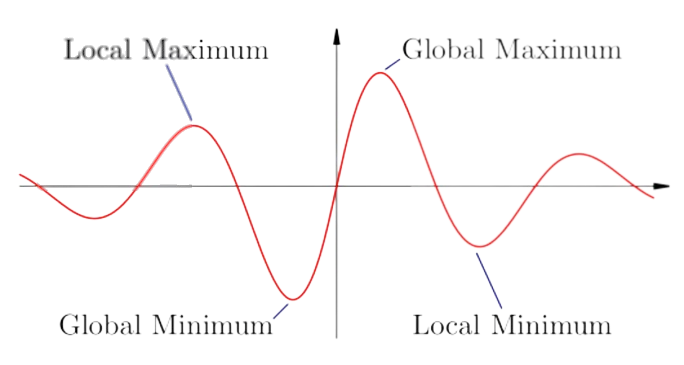
\includegraphics[width = 0.95\textwidth, height = 3cm]{img/extrema.png}
    
\end{frame}

% \begin{frame}{The monotonicity of a function according to its derivative}

%     \begin{block}{Increasing and decreasing according to the derivative}

%         \begin{enumerate}[leftmargin = 0.5cm, label = $\bullet$, rightmargin = 0.2cm]
        
%         \item $\blue{f'(x) \geq 0}$ ($\orange{f'(x) \leq 0}$) for all $x\in I\subset\R \Longrightarrow f$ is \blue{increasing} (\orange{decreasing}) in $I$

%         \item $f'(x) = 0$ for all $x$ in an \red{open interval} $I\subset\R \Longrightarrow f$ is constant (monotone) in $I$
        
%         \end{enumerate}

%         If the inequalities are strict, $f$ is said to be strictly \blue{increasing} (\orange{decreasing})
        
%     \end{block}

%     \red{Note} that we asked for $I$ to be an open interval. This is to avoid $I$ being a single point, since it is not generally true that $f'(x) = 0$ implies that $f$ is monotonic at $x = a$. \\ \textbf{Example:} $f(x) = x^3$ at $x = 0$
%     \vspace{0.3cm}
    
%     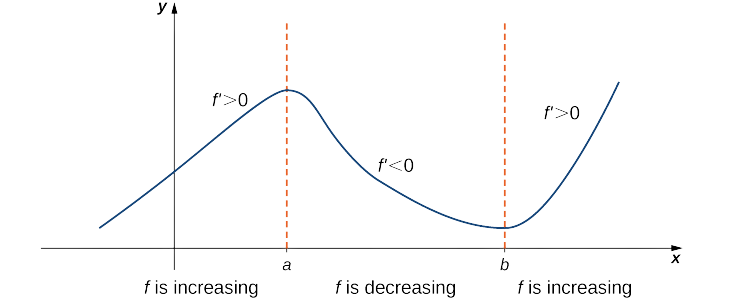
\includegraphics[width = \textwidth, height = 3.3cm]{img/increasing.decreasing.derivative.png}
    

% \end{frame}

\begin{frame}{Critical points of a function}
    \vspace{0.2cm}
    
    Those points where $f'(x) = 0$, along with the points where $f'(x)$ is not defined, \textbf{play a critical role in optimization}, so they are called \textbf{critical points}
    
    \begin{block}{Critical points of a function}
        
        $x = a$ is called a \textbf{critical point} of $f$ iff either

        \begin{enumerate}[leftmargin = 0.8cm, label = (\textit{\roman*}), rightmargin = 0.2cm]
            
            \item $f$ is differentiable at $x = a$ and $f'(a) = 0$, or
            
            \item $f$ is not differentiable at $x = a$

        \end{enumerate}
        
    \end{block}
    \vspace{0.2cm}
    
    \centering
    \textbf{Examples of critical points}
    \vspace{-0.1cm}
    
    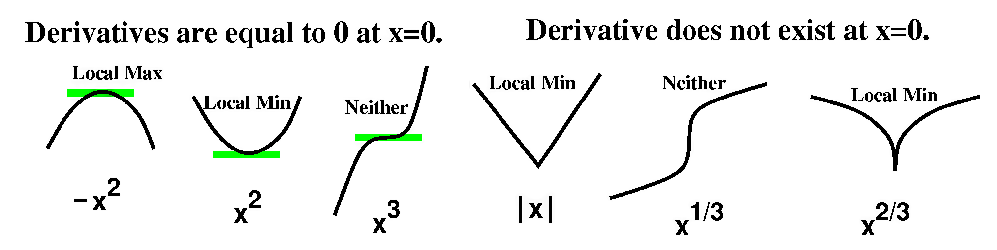
\includegraphics[width = 0.9\textwidth]{img/critical-points.png}

    

\end{frame}

\begin{frame}{Finding extremes by means of the (first) derivative}

    \begin{block}{Necessary condition for local extreme points}

        Suppose that $f$ is differentiable on an open interval $I$. Then,
        \vspace{-0.1cm}
        
        \begin{center}
            $a \in I$ is a maximum or minimum point for $f \Longrightarrow a$ is a \textbf{critical point} for $f$    
        \end{center}
        
        
    \end{block}

    \begin{block}{Sufficient condition for local extreme points. The first-derivative test}

    Suppose that $f(x)$ is derivable on an open interval $I$ containing the point $x = a$, except possibly at $x = a$. Then, if
    \vspace{-0.1cm}

    \begin{enumerate}[leftmargin = 0.8cm, label = (\textit{\roman*}), rightmargin = 0.2cm]
        
        \item $a\in I$ is a critical point for $f$, and

        \item \blue{$f'(x) \geq 0$} (\orange{$f'(x) \leq 0$}) for all $x\in I$ such that $x < a$, and
        
        \item \blue{$f'(x) \leq 0$} (\orange{$f'(x) \geq 0$}) for all $x\in I$ such that $x > a$
        
    \end{enumerate}
        
    Then $a$ is a local \blue{maximum} (\orange{minimum}) point for $f$
        
    \end{block}
    
\end{frame}

\begin{frame}{Visualizing the first-derivative test}

    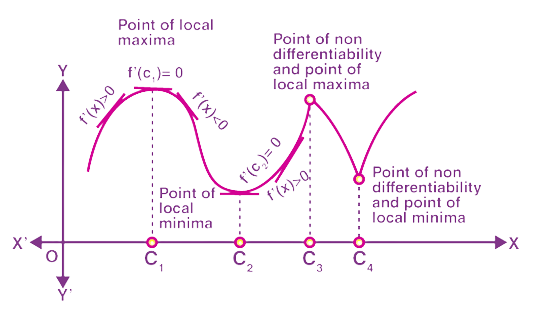
\includegraphics[width = \textwidth]{img/first-derivative-test.png}
    
\end{frame}

\begin{frame}{The first-derivative-test methodology to find \orange{local} extremes. An example}

    {\hspace{0.4cm}
    \textbf{Find the \orange{local} extreme points} of the function \href{https://www.desmos.com/calculator/a6rnvzud0w}{$f(x) = \frac{x^2}{x - 1}$} with domain $\R\backslash\{1\}$
    }
    
    \begin{enumerate}[leftmargin = 0.5cm, label = , rightmargin = 0.2cm]

        \item \textbf{Step 1: Find} $\pmb{f'(x)}$.

        We apply the quotient rule to obtain $f'(x) = \frac{x^2 - 2x}{(x - 1)^2}$

        \item \textbf{Step 2: Find all critical points and all values where $\pmb{f}$ is not defined}

        $f'(x) = 0 \Leftrightarrow x = 0, x = 2$ \\
        $f'(x)$ is not defined at $x = 1$ \\
        $f(x)$ is not defined at $x = 1$

        \item \textbf{Step 3: Analyze intervals of decrease or increase}

        \begin{table}
        \begin{flushleft}
        \begin{tabular}{r|lll}
            interval        & sample $x$-value  & $f'(x)$ & monotonicity \\ \hline
            $(-\infty, 0)$  & $x = -1$          & $f'(-1) = 3/2 > 0$    & $f$ increases \\
            $(0, 1)$        & $x = 1/2$         & $f'(1/2) = -3 < 0$     & $f$ decreases \\
            $(1, 2)$        & $x = 3/2$         & $f'(3/2) = -3 < 0$     & $f$ decreases \\
            $(2, \infty)$   & $x = 3$         & $f'(3) = 3/4 > 0$     & $f$ increases
        \end{tabular}
        \end{flushleft}
        \end{table}
        

        \item \textbf{Step 4: Find the local extreme points}
        
        We are looking for points where $f$ is defined and $f'$ changes sign.

        $x = 0$ is a point of local maximum and $x = 2$ is a point of local minimum

    \end{enumerate}
    
\end{frame}

\begin{frame}{Finding \orange{global} extremes in an \blue{closed interval}. An example}

    {\hspace{0.1cm}
    \textbf{Find the \orange{global} extreme points} of \href{https://www.desmos.com/calculator/s3vwtug8pu}{$f(x) = 2x^3 + 3x^2 - 12x$} over the interval $[-3, 3]$
    }
    
    \begin{enumerate}[leftmargin = 0.2cm, label = , rightmargin = 0.1cm]

        \item \textbf{Step 1: Find} $\pmb{f'(x)}$.

        $f'(x) = 6(x+2)(x-1)$

        \item \textbf{Step 2: Find all critical points and all values where $\pmb{f}$ is not defined}

        The critical points are $x = -2$ and $x = 1$

        \item \textbf{Step 3: Analyze intervals of decrease or increase}

        \begin{table}
        \begin{flushleft}
        \begin{tabular}{r|lll}
            interval    & sample $x$-value  & $f'(x)$               & monotonicity \\ \hline
            $(-3, -2)$  & $x = -5/2$        & $f'(-5/2) = 21/2 > 0$ & $f$ increases \\
            $(-2, 1)$   & $x = 0$           & $f'(0) = -12 < 0$      & $f$ decreases \\
            $(1, 3)$    & $x = 2$           & $f'(2) = 24 > 0$      & $f$ increases
        \end{tabular}
        \end{flushleft}
        \end{table}

    \end{enumerate}

        \begin{minipage}{0.53\textwidth}
            
            \begin{enumerate}[leftmargin = 0.2cm, label = , rightmargin = 0.1cm]
            
            \item \textbf{Step 4: Find the local extreme points \\ 
            (look also at the interval's end-points)}
        
            \begin{table}
            \begin{flushleft}
            \begin{tabular}{c|cccc}
                $x$     & $f(x)$    & before    & after     & min/max? \\ \hline
                $-3$    & $9$       & $-$        & $\nearrow$  & minimum  \\
                $-2$    & $20$      & $\nearrow$  & $\searrow$  & maximum  \\
                $1$     & $-7$      & $\searrow$  & $\nearrow$  & minimum  \\
                $3$     & $45$      & $\nearrow$  & $-$        & maximum
            \end{tabular}
            \end{flushleft}
            \end{table}
            
            \end{enumerate}
            
        \end{minipage}
        \begin{minipage}{0.43\textwidth}
            \vspace{-1.59cm}
            
            \begin{enumerate}[leftmargin = 0.2cm, label = , rightmargin = 0.1cm]
            
            \item \textbf{Step 5: Compare local extremes to find the global extremes}

            $\bullet$ $(1, -7)$ is the global minimum \\ 
            $\bullet$ $(3, 45)$ is the global maximum
        
            \end{enumerate}
            
        \end{minipage}
    
\end{frame}

\begin{frame}{Finding \orange{global} extremes in the \blue{whole domain}. An example}

    {\hspace{0.1cm}
    \textbf{Find the \orange{global} extreme points} of \href{https://www.desmos.com/calculator/1a5ijpy9x7}{$f(x) = xe^{3x}$} over \blue{$\R$}
    }
    
    \begin{enumerate}[leftmargin = 0.2cm, label = , rightmargin = 0.1cm]

        \item \textbf{Step 1: Find} $\pmb{f'(x)}$.

        $f'(x) = e^{3x}(1 + 3x)$

        \item \textbf{Step 2: Find all critical points and all values where $\pmb{f}$ is not defined}

        The only critical point is $x = -1/3$

        \item \textbf{Step 3: Analyze intervals of decrease or increase}

        \begin{table}
        \begin{flushleft}
        \begin{tabular}{r|lll}
            interval            & sample $x$-value  & $f'(x)$               & monotonicity \\ \hline
            $(-\infty, -1/3)$   & $x = -1$          & $f'(-1) = -2/e^3 < 0$ & $f$ decreases \\
            $(-1/3, \infty)$    & $x = 0$           & $f'(0) = 1 > 0$        & $f$ increases
        \end{tabular}
        \end{flushleft}
        \end{table}

    \end{enumerate}

        \begin{minipage}{0.66\textwidth}
            
            \begin{enumerate}[leftmargin = 0.2cm, label = , rightmargin = 0.1cm]
            
            \item \textbf{Step 4: Find the local extreme points and \\
            the limits of $f$ at the boundary points of its domain}
        
            \begin{table}
            \begin{flushleft}
            \begin{tabular}{c|cccc}
                  & $f(x)$ or  &  &    &\\ 
                $x$     & $\lim_{y\rightarrow x} f(y)$ & before    & after     & min/max? \\ \hline
                $-\infty$    & $0$       & $-$        & $\searrow$  & ``maximum''  \\
                $-1/3$    & $-(3e)^{-1}$      & $\searrow$  & $\nearrow$  & minimum  \\
                $\infty$     & $\infty$      & $\nearrow$  & $-$  & ``maximum''
            \end{tabular}
            \end{flushleft}
            \end{table}
            
            \end{enumerate}
            
        \end{minipage}
        \begin{minipage}{0.31\textwidth}
            \vspace{-0.25cm}
            
            \begin{enumerate}[leftmargin = 0.2cm, label = , rightmargin = 0cm]
            
            \item \textbf{Step 5: Compare local extremes and limit values to find global extremes}

            \item $\bullet$ $(-1/3, -1/(3e))$ \\ 
            is the global minimum \\ 
            $\bullet$ There is no global maximum
        
            \end{enumerate}
            
        \end{minipage}
    
\end{frame}

\begin{frame}{The convexity of a function and its extreme values}
    
    \vspace{0.2cm}
    
    \begin{block}{Extreme values and convexity}

        Let $f(x)$ be a function defined in the interval $I\subset \R$, and 
        $x = a$ be a critical point for $f(x)$ in the interior of $I$. Then,

        \begin{enumerate}[leftmargin = 0.5cm, label = $\bullet$, rightmargin = 0.2cm]
        
        \item If $f(x)$ is \blue{convex} (\orange{concave}), then $x = a$ is a \blue{minimum} (\orange{maximum}) point for $f(x)$ in $I$

        \item If $f(x)$ is strictly \blue{convex} (\orange{concave}), then $x = a$ is its \textbf{unique} \blue{minimum} (\orange{maximum}) point in $I$

        \end{enumerate}
        
    \end{block}

    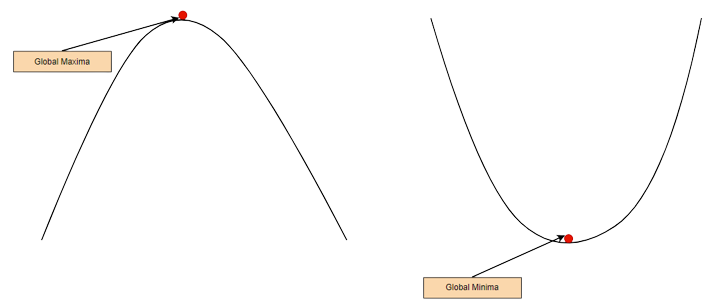
\includegraphics[width = 0.95\textwidth, height = 4.5cm]{img/convexity-unique-extremes.png}
    
\end{frame}

\begin{frame}{Finding extremes by means of the second derivative}

    \begin{block}{Sufficient condition for local extreme points. The second-derivative test}

    Suppose that $f(x)$ is twice derivable on an open interval $I$ containing the point $x = a$. %, except possibly at $x = a$.
    Then
    \vspace{-0.1cm}

    \begin{enumerate}[leftmargin = 0.8cm, label = (\textit{\roman*}), rightmargin = 0.2cm]

        \item $f'(a) = 0$ and \blue{$f''(a) > 0$} (\orange{$f''(a) < 0$}) $\Longrightarrow$ $x = a$ is a strict local \blue{maximum} (\orange{minimum}) point
        
        \item $f'(a) = 0$ and $f''(a) = 0 \Longrightarrow x = a$ could be a local maximum, a local minimum, or neither
        
    \end{enumerate}
        
    Then $a$ is a local \blue{maximum} (\orange{minimum}) point for $f$
        
    \end{block}

    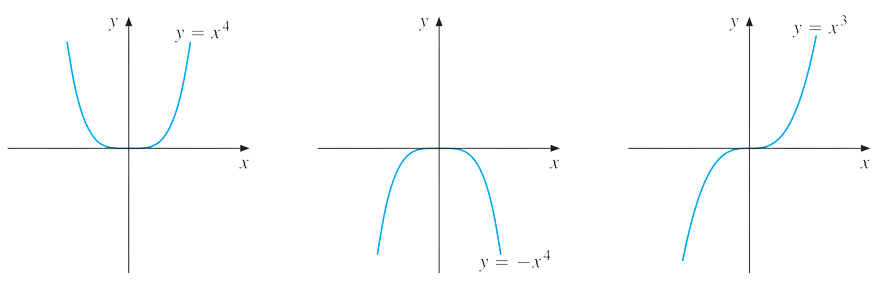
\includegraphics[width = \textwidth]{img/min-max-inflexion.png}
    
\end{frame}

\begin{frame}{The Extreme Value Theorem}

    \centering
    \textbf{Does a function actually attain global minima or maxima values?}

    \begin{block}{The Extreme Value Theorem (EVT)}
        \begin{minipage}{0.4\textwidth}
            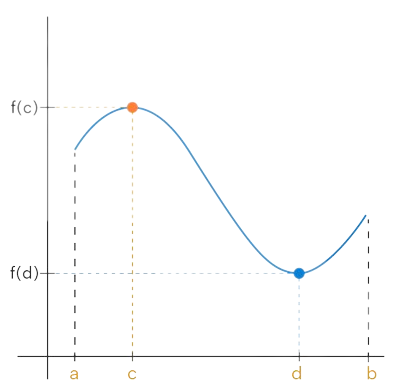
\includegraphics[width = \textwidth]{img/extreme-value-theorem.png}
        \end{minipage}
        \begin{minipage}{0.55\textwidth}
            Let $f$ be a continuous function defined on a closed interval $[a, b]$. Then, there exist points $c, d \in [a, b]$ where $f$ reaches its maximum and minimum values. respectively. \\ 
            That is,
            % \begin{align*}
            $$
            f(c) \geq f(x) \geq f(d) \text{ for all } x\in[a, b]
            $$
            % \end{align*}
            % \vspace{0.4cm}
            \textbf{Note} that the extreme value theorem is a sufficient condition for a function to attain its extremes, not a necessary one
        \end{minipage}
        
        
    \end{block}
    
\end{frame}

\begin{frame}{Economical application: The Profit Maximization Principle}

    \begin{enumerate}[leftmargin = 0.3cm, label = , rightmargin = 0.2cm]

        \item \textbf{Profit as a function of quantity:} $\Pi(q) = C(q) - R(q) = $ how much a company makes, in net terms, by producing $q$ units of a product and selling them at $P(q)$ dollars each unit

        \item \textbf{Question:} How much should the company produce to maximize profits?

        \item \textbf{Assumptions:} In practice, it is sensible to assume the following conditions:
        
        \begin{enumerate}[leftmargin = 0.3cm, label = (\textit{\roman*}), rightmargin = 0.2cm]

            \item \orange{Economy:} The company has a maximum production capacity \\
                  \blue{Maths:} The domain of $\Pi$ is $[0, L]$, for some $L > 0$

            \item \orange{Economy:} The profit smoothly depends on the quantity \\
                  \blue{Maths:} $\Pi$ is derivable

            \item \orange{Economy:} The optimal strategy is neither none production nor full production \\
                  \blue{Maths:} $q = 0$ and $q = L$ are not maximum points for $\Pi$
                
        \end{enumerate}

        \item \textbf{Conclusions:}

        \begin{enumerate}[leftmargin = 0.3cm, label = (\textit{\roman*}), rightmargin = 0.2cm]

            \item \blue{Maths:} The EVT guarantees that $\Pi$ attains its maximum at some point $\overline{q} \in (0, L)$ \\
            {\hspace{1cm} The first-derivative test guarantees that}
            \vspace{-0.1cm}
            $$
            \blue{\Pi'(\overline{q}) = R'(\overline{q}) - C'(\overline{q}) = 0}
            $$
            \vspace{-0.55cm}
            
            \orange{Economy:} The Profit Maximization Principle
            \vspace{0.07cm}
            
            \centering
            \orange{\textit{The optimum production level occurs when \\ the marginal revenue equals the marginal cost}}
        

        \end{enumerate}
        
    \end{enumerate}
    
\end{frame}
%----------------------- OPTIMIZATION 1D -----------------------%

%----------------------- DIFFERENTIAL CALCULUS 2D -----------------------%
% \section{Differential calculus of two-variables functions}

% \begin{frame}{Functions of two variables}

%     Recall that \textbf{functions can accept several variables}.
%     \vspace{0.3cm}

%     \textbf{Functions of two variables are of special importance} because they allow to illustrate how the theory and techniques of one-dimensional differential calculus extend to functions of many variables.
%     \vspace{0.3cm}
    
%     The class of bidimensional functions is also wide enough to find many applications in economics and other fields.
        
% \end{frame}

% \begin{frame}{Partial derivatives}

%     \textbf{Interpretation:} Partial derivatives measure the ("instantaneous") rate of change with respect to (w.r.t.) one variable when the other variables remain constant.
    
%     \begin{block}{Definition of partial derivatives}

%         For the function $f:\R^2\rightarrow\R$, with output $f(x, y)$,
%         \begin{enumerate}[leftmargin = 0.5cm, label = $\bullet$, rightmargin = 0.2cm]

%             \item $\frac{\partial f}{\partial x}$ is the function defined as
%             $$
%             \frac{\partial f}{\partial x}(x, y) := \lim_{h\rightarrow 0}\frac{f(x + h, y) - f(x, y)}{h},
%             $$
%             and is called \textbf{the partial derivative of} $\pmb{f}$ \textbf{w.r.t.} $\pmb{x}$.
            
%             \item $\frac{\partial f}{\partial y}$ holds an analogous definition and it is called the partial derivative of $f$ w.r.t. $y$.
            
%         \end{enumerate}
        
%     \end{block}

%     \begin{block}{Alternative notation}

%         $\partial_x f$ and $f_x$ are alternative notations of $\frac{\partial f}{\partial x}$.

%         $\partial_i f$ and $f_i$, for $i = 1, 2$, are commonly used to refer to the partial derivative w.r.t. the $i$th coordinate.
            
%         \end{block}
    
% \end{frame}

% \begin{frame}{Finding the partial derivative. An example}

%     \begin{block}{Example}
%     Compute the partial derivatives of $f(x, y) = x^4y + x^3y^2 + x^2 + y^5$.
%     \begin{enumerate}[leftmargin = 0.5cm, label = $\bullet$, rightmargin = 0.2cm]

%         \item $\frac{\partial f}{\partial x}(x, y) = 4x^3y + 3x^2y^2 + 2x$.

%         \item $\frac{\partial f}{\partial y}(x, y) = x^4 + 2x^3y + 5y^4$.
    
%     \end{enumerate}
%     \end{block}

%     \begin{block}{Example}
%     Compute the partial derivatives of $f(x, y) = xy/(x^2 + y^2)$.
%     \begin{enumerate}[leftmargin = 0.5cm, label = $\bullet$, rightmargin = 0.2cm]
        
%         \item Applying the quotient rule, we get
%         $$
%         \frac{\partial f}{\partial x}(x, y) = \frac{y(x^2 + y^2) - 2x^2y}{(x^2 + y^2)^2} = \frac{y^3 - x^2y}{(x^2 + y^2)^2}.
%         $$

%         \item Interchanging the roles of $x$ and $y$ we get the expression for $\frac{\partial f}{\partial x}(x, y)$
    
%     \end{enumerate}
%     \end{block}
    
% \end{frame}

% \begin{frame}{Economical application of partial derivatives: \\ Rate of change of production}

%     \textbf{The Cobb-Douglas production function} is defined by $q(k, l) = k^\alpha l^\beta$, for $\alpha, \beta > 0$. Variables $k$ and $l$ represent \textbf{capital} invested and \textbf{labour} input, respectively.
%     \vspace{0.3cm}

%     \textbf{Marginal product of capital}: $q_k(k, l) = \alpha k^{\alpha-1} l^\beta$

%     \textbf{Marginal product of labour}: $q_l(k, l) = \beta k^\alpha l^{\beta-1}$
%     \vspace{0.3cm}
    
%     \begin{enumerate}[leftmargin = 0.5cm, label = $\bullet$, rightmargin = 0.2cm]
    
%     \item What is the approximate increase in production when the capital slightly changes and the labour is held constant?
%     $$
%     q(k + \Delta k, l) - q(k , l) \approx q_k(k, l)\Delta k.
%     $$
%     % \vspace{0.3cm}
    
%     \item What is the approximate increase in production when the labour marginally changes and the capital is held constant?
%     $$
%     q(k, l + \Delta l) - q(k , l) \approx q_k(k, l)\Delta l.
%     $$
%     \end{enumerate}
    
% \end{frame}

% % \begin{frame}{Contours and implicit functions.}

% %     \begin{block}{Definition of contours and implicit functions}
% %         Consider the function $f(x, y)$ and a constant $c\in\R$. 
% %         \begin{enumerate}[leftmargin = 0.5cm, label = $\bullet$, rightmargin = 0.2cm]
% %             \item The set $\{(x, y)\ :\ f(x, y) = c\}$ is called the \textbf{contour of level} $\pmb{c}$ (or $c$-contour) of $f$.

% %             \item The equation $f(x, y) = c$ is said to implicitly define $y$ as a function of $x$, if the $c$-contour of $f$ can be seen as the graph of a function of $x$, $y(x)$.
% %         \end{enumerate}
        
% %     \end{block}
    
% % \end{frame}

% % \begin{frame}{The bidimensional chain rule}

% % Suppose that, in the production function $q(k , l)$, the capital and labour are also functions of time. That is, $k = k(t)$ and $l = l(t)$, for $t\in\R_+$.
% % \vspace{0.2cm}

% % \textbf{Question:} what is the (``instantaneous'') rate of change of the production w.r.t. the time? That is, $Q'(t)$, with $Q(t) = q(k(t), l(t))$.
% % \vspace{0.2cm}

% % This illustrates the necessity of analyzing the derivative of a bidimensional function with respect to an exogenous variable.

% % \begin{block}{The chain rule}
% %     Consider the functions $x(t)$, $y(t)$ and $f(x, y)$. Assume that the composition $F(t) = f(x(t), y(t))$ can be made. Then,
% %     $$
% %     F'(t) = \frac{\partial f}{\partial x}(x(t), y(t))x'(t) + \frac{\partial f}{\partial y}(x(t), y(t))y'(t)
% %     $$
% % \end{block}
    
% % \end{frame}

% % \begin{frame}{Economic application of the chain rule: \\ The production as a function of time}

% %     \begin{block}{Problem}
% %     At time $t\in\R_+$, the capital invested and labour input of a company are given by
% %     $$
% %     k(t) = 4 + 0.1t, \quad l(t) = 9 - 0.05t^2.
% %     $$
% %     We know that the production function is given by $q(k, l) = k^2l$. How does a small change in time affect production?
% %     \end{block}

% %     \textbf{Solution:}
% %     \begin{enumerate}[leftmargin = 0.5cm, label = \arabic*., rightmargin = 0.2cm]
% %     \item Compute the partial derivatives of $q$ and the derivatives of $k$ and $l$:
% %     $$
% %     q_k(k, l) = 2kl,\; q_l(k, l) = k^2,\; k'(t) = 0.1,\; l'(t) = -0.1t.
% %     $$
% %     \item By applying the chain rule and considering $Q(t) = q(k(t), l(t))$, we get
% %     \begin{align*}
% %     Q'(t) &= q_k(k(t), l(t))k'(t) + q_l(k(t), l(t))l'(t) \\
% %     &= 2(4 + 0.1t)(9 - 0.05t^2)0.1 - (4 + 0.1t)^2 0.1t
% %     \end{align*}
% %     \end{enumerate}
    
% % \end{frame}

% \begin{frame}{Second-order partial derivatives}

%     For the function $f(x, y)$, note that $f_x$ and $f_y$ are also functions of two variables, so we can obtain their partial derivatives. They are called \textbf{second-order partial derivatives} of $f$, denoted by
%     $$
%     \frac{\partial^2 f}{\partial x^2} := \frac{\partial f_x}{\partial x},\quad
%     \frac{\partial^2 f}{\partial y^2} := \frac{\partial f_y}{\partial y},\quad
%     \frac{\partial^2 f}{\partial x\partial y} := \frac{\partial f_x}{\partial y},\quad
%     \frac{\partial^2 f}{\partial y\partial x} := \frac{\partial f_y}{\partial x}.
%     $$

%     \begin{block}{Alternative notation}

%         \begin{enumerate}[leftmargin = 0.5cm, label = $\bullet$, rightmargin = 0.2cm]
%         \item $\partial_{x^2} f$ and $f_{xx}$ are alternative notations of $\frac{\partial^2 f}{\partial x^2}$.

%         \item $\partial_{xy} f$ and $f_{xy}$ are alternative notations of $\frac{\partial^2 f}{\partial x\partial y}$.

%         \item $\partial_{ij} f$ and $f_{ij}$, for $i, j = 1, 2$, are commonly used to refer to the second-order partial derivative w.r.t. the $i$th and $j$th coordinate.
%         \end{enumerate}
            
%     \end{block}
    
% \end{frame}
% %----------------------- DIFFERENTIAL CALCULUS 2D -----------------------%

% %----------------------- OPTIMIZATION 2D -----------------------%
% \section{Optimization of two-variables functions}

% \begin{frame}{Maxima, minima, and saddle points}

%     \textbf{Convex set:} A set $S$ in the plane is convex if every segment connecting each pair of points in $S$ is contained in $S$. 
%     \vspace{0.2cm}
    
%     Consider the function $f(x, y)$ with convex domain $S\subset \R^2$
%     \vspace{0.2cm}
    
%     \textbf{Critical points:} $(a, b)$ is a critical point for $f$ if either $f_x(a, b) = f_y(a, b) = 0$ or one of the partial derivative do not exist at $(a, b)$.

%     \begin{block}{First-order necessary condition for extremes}

%         If the point $(a, b)$ in the interior of $S$ is a local minimum or a local maximum for $f$, then it is a critical point of $f$.
        
%     \end{block}

%     The reverse condition does not hold, as a critical point can be a \textbf{saddle point}
    
% \end{frame}

% \begin{frame}{Visualizing extremes}

%     \begin{minipage}{0.47\textwidth}
%         \centering
%         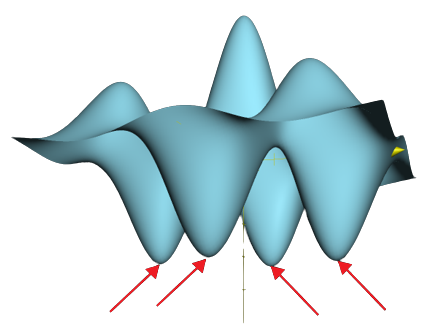
\includegraphics[width = \textwidth]{img/local-minima.png}
%         % \vspace{0.1cm}
        
%         {\hspace{0.5cm} \Large These are local minima}
%     \end{minipage}
%     \begin{minipage}{0.47\textwidth}
%         \vspace{-1.1cm}
        
%         \centering
%         {\hspace{0.5cm} \Large These are local maxima}
%         \vspace{0.2cm}
        
%         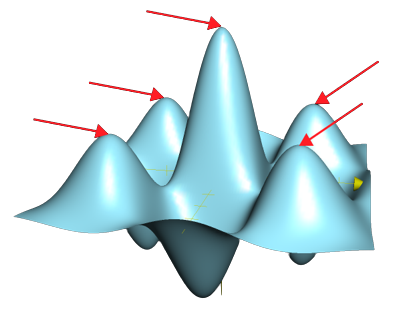
\includegraphics[width = \textwidth]{img/local-maxima.png}
%     \end{minipage}
    
% \end{frame}

% \begin{frame}{Visualizing first-order necessary condition}


% \centering
% The first-order condition ensures the tangent planes to be horizontal at the extrema.

% 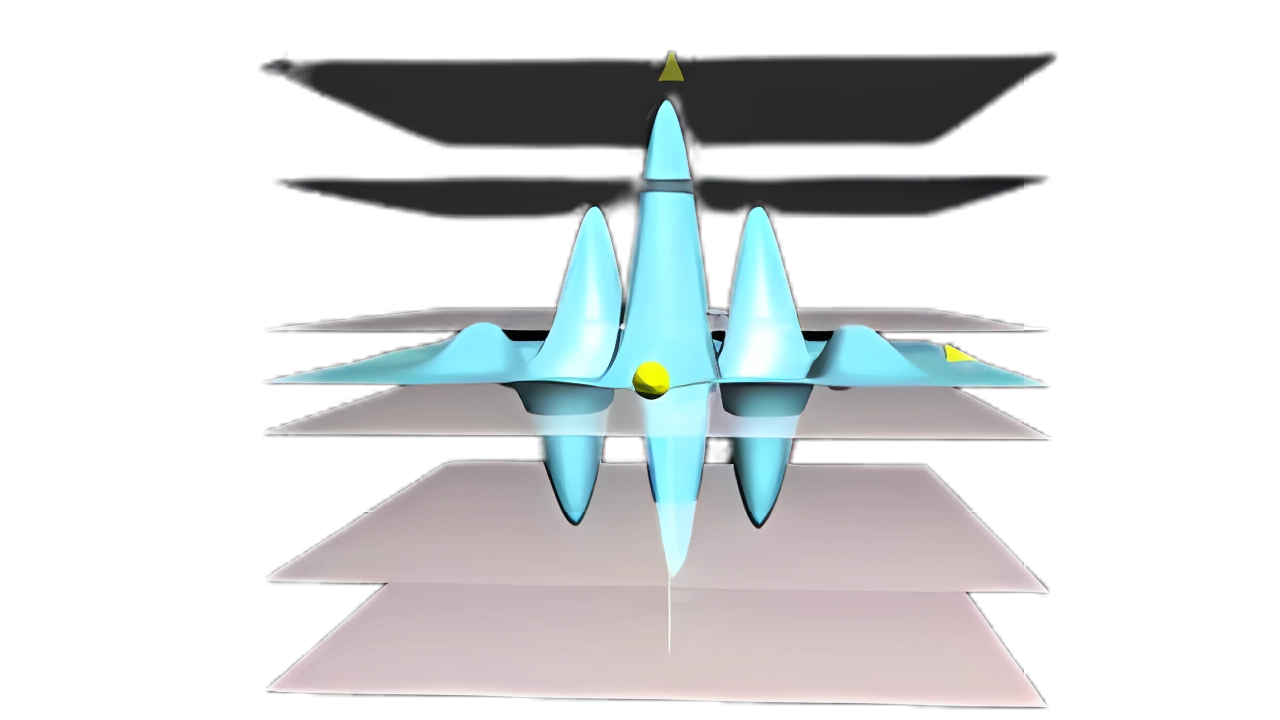
\includegraphics[width = 0.9\textwidth]{img/tangent-planes.png}
    
% \end{frame}

% \begin{frame}{Visualizing saddle points}

%     \begin{minipage}{0.4\textwidth}
%         \textbf{Saddle point:} The function has a local minimum in one coordinate and a local maximum in the other coordinate
%     \end{minipage}\hspace{0.2cm}
%     \begin{minipage}{0.56\textwidth}
%     \begin{center}
%         \centering
%         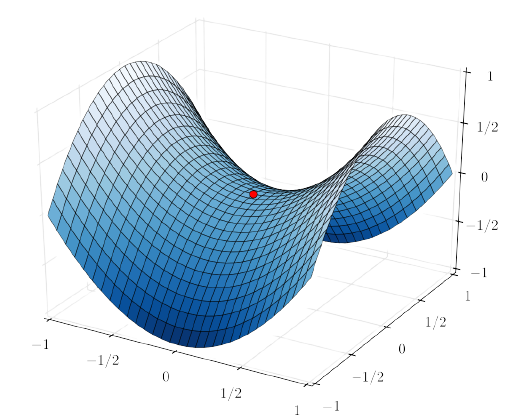
\includegraphics[width = \textwidth, height = 4cm]{img/saddle_point.png}    
%     \end{center}
%     \end{minipage}
%     \vspace{0.1cm}

%     \begin{minipage}{0.4\textwidth}
%         \centering
%         Mathematicians named it ``saddle point'' for its similarity to a saddle
%         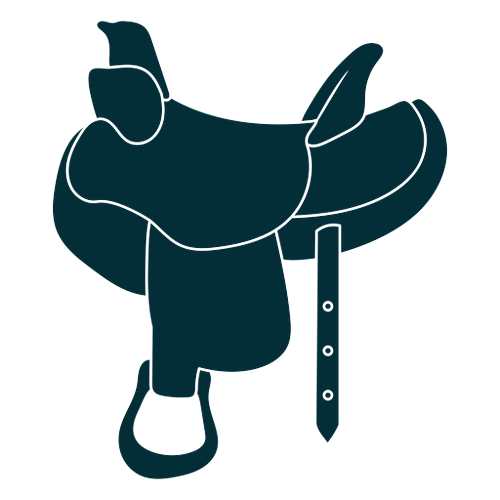
\includegraphics[width = 0.9\textwidth, height = 3cm]{img/saddle.png}  
%     \end{minipage}\hspace{0.6cm}
%     \begin{minipage}{0.5\textwidth}
%         \centering
%         It might have been called ``Pringles point'', had it been discovered in modern times.
%         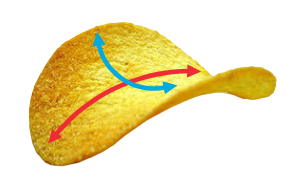
\includegraphics[width = 0.8\textwidth, height = 3cm]{img/pringles.png}  
%     \end{minipage}
    
    
% \end{frame}

% \begin{frame}{The second partial derivative test}

%     Fortunately, there is a test based on second-order partial derivatives to identify if a critical point (where the partial derivatives exist) is a local minimum, a local maximum, or a saddle point.
    
%     \begin{block}{The second partial derivative test}

%         Let $f(x, b)$ be a function in the convex domain $S\subset\R^2$, and $(a, b)$ an interior point of $S$ which is a critical point of $f$. Assume that $f$ is twice continuously differentiable.

%         Consider $D = f_{xx}(a, b)f_{yy}(a, b) - f_{xy}(a, b)^2$. Then,
%         \begin{enumerate}[leftmargin = 0.5cm, label = $\bullet$, rightmargin = 0.2cm]
%             \item If $D < 0$, then $(a, b)$ is a saddle point
%             \item If $D > 0$, then $(a, b)$ is an extreme, and
%             \begin{enumerate}[leftmargin = 0.5cm, label = (\textit{\roman*}), rightmargin = 0.2cm]
%                 \item If $f_{xx}(a, b) < 0$, then $(a, b)$ is a local maximum point
%                 \item If $f_{xx}(a, b) > 0$, then $(a, b)$ is a local minimum point
%             \end{enumerate}
%         \end{enumerate}
%         If $D = 0$ the second derivatives alone cannot tell us whether $f$ has a local minimum or maximum at $(a, b)$.

%     \end{block}
       
% \end{frame}

% \begin{frame}{The second partial derivative test. The methodology}

%     {\hspace{0.4cm}
%     \textbf{Find the \orange{global} extrema} of the function \href{https://www.desmos.com/3d/2803979607}{$f(x, y) = x^4 - 4x^2 + y^2$} with domain $\R^2$.
%     }
    
%     \begin{enumerate}[leftmargin = 0.5cm, label = , rightmargin = 0.2cm]

%         \item \textbf{Step 1: Find the partial derivatives} 
        
%         $f_x(x, y) = 4x^3 - 8x$, $f_y(x, y) = 2y$.

%         \item \textbf{Step 2: Find the critical points}

%         $f_x(x, y) = f_y(x, y) = 0 \Leftrightarrow (x, y) \in\{(0, 0), (\sqrt{2}, 0), (-\sqrt{2}, 0)\}$

%         \item \textbf{Step 3: Find the second partial derivatives and the determinant of the Hessian}

%         $f_{xx}(x, y) = 12x^2 - 8$, $f_{yy}(x, y) = 2$, $f_{xy}(x, y) = 0$\\
%         $D(x, y) = f_{xx}(x, y)f_{yy}(x, y) - f_{xy}(x, y)^2 = 2(12x^2 - 8)$
        
%         \item \textbf{Step 4: Apply the second derivative test}

%         \begin{table}
%         \begin{flushleft}
%         \begin{tabular}{r|lll}
%             $(x, y)$        & $H(x, y)$ & $f_{xx}(x, y)$& classification\\ \hline
%             $(0, 0)$        & $-16 < 0$     & -8           & saddle point  \\
%             $(\sqrt{2}, 0)$ & $32 > 0$      & $16> 0$         & local minimum \\
%             $(-\sqrt{2}, 0)$& $32 > 0$     & $16 > 0$         & local minimum
%         \end{tabular}
%         \end{flushleft}
%         \end{table}

%         \item \textbf{Step 5: Compare all local extrema to find the global}

%         $f(\pm\sqrt{2}, 0) = -4 \Longrightarrow (\pm\sqrt{2}, 0)$ are both global minima. \\
%         The function does not have a global maximum.

%     \end{enumerate}

% \end{frame}

% \begin{frame}{Economic application: two-products monopoly profit maximization}

%     A firm has a monopoly for the manufacture of two products, $X$ and $Y$, for which the (inverse) demand functions are
%     $$
%     p_X = 6 - x,\quad p_Y = 16 - 2y,
%     $$
%     where $x$ and $y$ are the quantities of $X$ and $Y$, and $p_X$ and $p_Y$ are the respective prices. The firm's cost function is $C(x,y) = x^2/2 + y^2/2 + xy$. Determine the output quantities which will maximize the firm's profit, and calculate the maximum profit.
    
% \end{frame}

% \begin{frame}{Two-products monopoly profit maximization - Solution}

% \small
% {
% \hspace{0.12cm}
% \textbf{Goal:} Maximize profit $\;\pi(x,y)=p_X x+p_Y y - C(x,y) = \href{https://www.desmos.com/3d/dvr5ho9xry}{6x-\tfrac{3}{2}x^2-xy+16y-\tfrac{5}{2}y^2}$ %with
% %$p_X=6-x,\; p_Y=16-2y,\; C(x,y)=\tfrac{x^2}{2}+\tfrac{y^2}{2}+xy$.
% }

% \begin{enumerate}[leftmargin=0.2cm, label=, rightmargin=0.2cm]

% \item \textbf{Step 1: Partial derivatives}
% $$
% \pi_x=6-3x-y,\quad \pi_y=16-x-5y.
% $$

% \item \textbf{Step 2: Critical points} \quad
% Solve $\pi_x=\pi_y=0$:
% \[
% \begin{cases}
% 6-3x-y=0\\
% 16-x-5y=0
% \end{cases}
% \Longrightarrow (x,y)=(1,3).
% \]

% \item \textbf{Step 3: Second partials and determinant of Hessian}
% \[
% \pi_{xx}=-3,\;\pi_{yy}=-5,\;\pi_{xy}=-1,
% \quad
% D=\pi_{xx}\pi_{yy}-\pi_{xy}^2=(-3)(-5)-(-1)^2=14>0.
% \]
% % (Hessian matrix $\,\begin{pmatrix}-3&-1\\-1&-5\end{pmatrix}$.)

% \item \textbf{Step 4: Second derivative test}
% \[
% D>0 \ \text{and} \ \pi_{xx}=-3<0 \ \Rightarrow\ (1,3)\ \text{is a local maximum.}
% \]

% \item \textbf{Step 5: Global conclusion \& optimal value} \\
% $$
% \lim_{x\rightarrow\pm\infty}\pi(x,y) = \lim_{y\rightarrow\pm\infty}\pi(x,y) = -\infty\; \Rightarrow
% \text{the only local max is also \textbf{global}}.
% $$
% \vspace{0.1cm}

% \textbf{Max profit:} 
% $
% \pi^*=\pi(1,3)=27.
% $

% \end{enumerate}
% \end{frame}



%----------------------- OPTIMIZATION 2D -----------------------%

%----------------------- SUMMARY -----------------------%
% \section{Summary}

% \begin{frame}{Summary. Precalculus}

%     \begin{block}{Main concepts. Precalculus}
%         \begin{enumerate}[leftmargin = 0.5cm, label = $\bullet$, rightmargin = 0.2cm]
%             \item Limits of functions, left-right limits
%             \item Analytical properties of functions: continuity, monotonicity, convexity
%             \item Rules of limits, determinate and indeterminates forms
%     \end{enumerate}
%     \end{block}
    
% \end{frame}

% \begin{frame}{Summary. Differential Calculus and Optmization}

%     \begin{block}{Differential calculus}
%         \begin{enumerate}[leftmargin = 0.5cm, label = $\bullet$, rightmargin = 0.2cm]
%             \item The derivative of a function 
%             \item Rules to compute derivatives and derivatives of common functions
%             \item Monotonicity according to derivatives
%             \item Economic applications: Marginal cost and Elasticity of demand
%             \item The L'Hôspital rule for indeterminate forms of limits
%             \item Higher order derivatives
%             \item Convexity and second order derivatives
%     \end{enumerate}
%     \end{block}

%     \begin{block}{Optimization}
%         \begin{enumerate}[leftmargin = 0.5cm, label = $\bullet$, rightmargin = 0.2cm]
%             \item Extreme and critical points
%             \item The first derivative test and its methodology
%             \item The extreme value theorem
%             \item Economic applications: Profit maximization
%     \end{enumerate}
%     \end{block}
    
% \end{frame}

% \begin{frame}{Summary. Two-variables Differential Calculus and Optimization}

%     \begin{block}{Differentiation of two-variables functions}
%         \begin{enumerate}[leftmargin = 0.5cm, label = $\bullet$, rightmargin = 0.2cm]
%             \item Partial derivatives
%             \item Economic application: Marginal production of capital and of labour
%             \item The bidimensional chain rule
%             \item Second-order partial derivatives
%     \end{enumerate}
%     \end{block}

%     \begin{block}{Optimization of two-variables functions}
%         \begin{enumerate}[leftmargin = 0.5cm, label = $\bullet$, rightmargin = 0.2cm]
%             \item Maxima, minima, and saddle points
%             \item The first-order necessary condition
%             \item The second partial derivative test and its methodology 
%     \end{enumerate}
%     \end{block}
    
% \end{frame}

%----------------------- SUMMARY -----------------------%

%----------------------- HISTORY -----------------------%
% \section{A brief of history about calculus}

% \begin{frame}{Roots of calculus}
    
% \end{frame}

% \begin{frame}{The calculus drama}
    
% \end{frame}

% \begin{frame}{Open Q\&A}

%     \centering Time to ask!
    
% \end{frame}
%----------------------- HISTORY -----------------------%


\end{document}
